\documentclass[%
 reprint,
%superscriptaddress,
%groupedaddress,
%unsortedaddress,
%runinaddress,
%frontmatterverbose, 
%preprint,
%preprintnumbers,
%nofootinbib,
%nobibnotes,
%bibnotes,
 amsmath,amssymb,
 aps,
prd,
%prb,
%rmp,
%prstab,
%prstper,
floatfix,
]{revtex4-2}

\usepackage{graphicx}% Include figure files
\usepackage{dcolumn}% Align table columns on decimal point
\usepackage{bm}% bold math
\usepackage{hyperref}% add hypertext capabilities
%\usepackage[mathlines]{lineno}% Enable numbering of text and display math
%\linenumbers\relax % Commence numbering lines

%\usepackage[showframe,%Uncomment any one of the following lines to test 
%%scale=0.7, marginratio={1:1, 2:3}, ignoreall,% default settings
%%text={7in,10in},centering,
%%margin=1.5in,
%%total={6.5in,8.75in}, top=1.2in, left=0.9in, includefoot,
%%height=10in,a5paper,hmargin={3cm,0.8in},
%]{geometry}

\begin{document}

\title{BUFF: Boosted Decision Tree based Ultra-Fast Flow matching}% Force line breaks with \\

\author{Cheng Jiang}
\email{C.Jiang-19@sms.ed.ac.uk}
 \affiliation{%
 School of Physics and Astronomy, University of Edinburgh, EH9 3FD, Edinburgh, United Kingdom
}%
\author{Sitian Qian}%
 \email{stqian@pku.edu.cn}
\affiliation{%
 School of Physics, Peking University, 100871, Beijing, China
}%

\author{Huilin Qu}
\email{huilin.qu@cern.ch}
\affiliation{
 CERN, EP Department, CH-1121 Geneva 23,  Switzerland
}



\date{\today}% It is always \today, today,
             %  but any date may be explicitly specified



\begin{abstract}
    Tabular data is one of the most frequently encountered data types in high energy physics. Unlike homogeneous data such as pixelated images, simulating high-dimensional tabular data while accurately capturing inter-variable correlations remains challenging, even with state-of-the-art architectures. Motivated by findings that tree-based models outperform deep learning models on tabular-data tasks, we adopt conditional flow matching and employ several techniques to integrate Gradient Boosted Trees as the regression backbone. Performance is evaluated across various tasks at different analysis levels using several public datasets. We demonstrate that training and inference for most high-level simulation tasks achieve speedups of orders of magnitude. The approach extends to low-level feature simulation and conditional generation with competitive performance.

\end{abstract}



\maketitle




\section{Introduction}\label{sec1}

Collisions at the Large Hadron Collider (LHC) \cite{lhc}, governed by quantum mechanics, are intrinsically probabilistic. This necessitates a vast number of simulated events to validate theoretical predictions. Large-scale Monte Carlo (MC) event production \cite{mc} relies on dedicated, often lengthy pipelines to perform Standard Model calculations. In the upcoming High-Luminosity LHC (HL-LHC) era \cite{hilhc}, these simulations will become even more CPU-intensive \cite{mcchallenge} given the much larger volume of data. It is therefore crucial to prevent limitations in physics output due to insufficient statistics arising from constrained computational budgets.


Deep generative models serving as fast surrogate simulators in collider physics enable rapid generation of particle collision data, drastically reducing the event generation time without sacrificing accuracy. Diffusion models (DMs) \cite{score,ddpm,diffusionbeatgan} excel at generating high-quality samples by iteratively denoising random noise, demonstrating strong performance in tasks such as fast calorimeter simulation \cite{calodiffu,caloscore,caloscore2,calocloud2,directdiff,pcjedi}. A common challenge of DM applications is that they only reach optimal performance after relatively long generation times. Many studies adopt distillation techniques such as progressive distillation and consistency models \cite{pd,cm,icm}. Normalizing flows (NFs) \cite{nfreview,inn}, on the other hand, stand out for their ability to model complex distributions efficiently, making them especially powerful for precise probability density estimation. Various generative models have been applied across a range of tasks \cite{calogan,calom,caloqvae,caloshowergan,deeptreegan}, including conditional phase space sampling \cite{madnis,madnis2,zunis,mm,nfeventgen,iflow,cqmnf}, fast shower generation \cite{caloflow,caloflow2,calopointflow2,l2flow,supercalo}, unfolding \cite{cinnfold,sbfold}, anomaly detection \cite{ad1,adben,nfad1,treead1}, and quark-gluon tagging \cite{qg}.

However, NFs intrinsically struggle to reach satisfactory performance in higher dimensions \cite{glow,fm}. Furthermore, most architectures adopted in high energy physics (HEP) are tailored for image synthesis. The majority of analysis-level observables are designed to be sensitive to specific phase space regions or to probe the substructure of hadronic objects. These variables exhibit shapes far more complex than a simple Gaussian and are naturally represented as tabular data. Simulating such high-dimensional tabular data while precisely capturing inter-variable correlations remains notably challenging with current approaches, particularly given the significantly longer training and validation times required for each analysis iteration.

Recently, conditional flow matching (CFM) \cite{cfm}, inspired by score matching diffusion models \cite{score} and optimal transport \cite{ot}, was introduced as a simulation-free approach that directly matches the vector field, demonstrating good scalability to very high dimensions. In this work, we build upon the technique introduced in~\cite{flowbdt}, which replaces the neural network backbone in CFM with Gradient Boosted Trees (GBT) \cite{bdt,gbt}, and apply it to particle physics for the first time. We name the overall methodology Boosted Decision Tree based Ultra-Fast Flow matching (BUFF), and refer to the specific model as flowBDT. Compared to~\cite{flowbdt}, our contributions include: (1)~the first application of tree-based flow matching to HEP datasets; (2)~the use of higher-order ODE solvers (Midpoint, Dormand-Prince) to reduce the number of required sampling steps; (3)~a multi-output tree strategy that provides a 5--8$\times$ speedup in inference; and (4)~conditional generation from non-Gaussian priors for unfolding and shower refinement. The rationale behind using tree-based CFM is that the vector fields and conditional probability paths generated from $N$-dimensional tabular data should also hold the similar structures inherent to them. Several comprehensive studies \cite{bdtbetter1,bdtbetter2} indicate that tree-based models surpass most of deep learning models in performance for tasks specific to tabular data, such as classification and regression. In Section~\ref{sec2}, we delve into the workings of the Tree-based Conditional Flow Matching and share some improved understanding of this method, alongside its novel applications. Section~\ref{sec3} describes the datasets utilized in our study. In Section~\ref{sec4}, we present the performance outcomes across various tasks using diverse datasets and a range of comprehensive metrics. Lastly, Section~\ref{sec5} offers potential applications and future directions for this line of research.



\section{Improved Understanding for Tree-based Flow matching}\label{sec2}

Suppose $f: \mathbb{R}^d \rightarrow \mathbb{R}^d$ is a continuously differentiable map between the target distribution $p_1$ and the base distribution $x \sim q_0$, which is typically a multidimensional Gaussian. Normalizing flow (NF) requires each composition of the inverse map $f(x) = f_{T-1}\circ...\circ f_{0}(x)$ to have valid Jacobian determinants during the sampling phase. By the change-of-variable rules, the log-likelihood loss for NF training is written as \cite{glow}:

\begin{subequations}
\begin{equation}
\begin{aligned}
    p_1(x_T) = q_0(f^{-1}(x_T)) \hspace{1mm} |\det[\frac{\partial f^{-1}}{\partial x_{t}}(x_T)]|\\
    = \frac{q_0(x)}{|\det[\frac{\partial f}{\partial x}(x)]|}, \hspace{4mm} x = f^{-1}(x_T)
\end{aligned}
\end{equation}
\begin{eqnarray}
    \log p_1(x_T) = \log q_0(x) - \sum_{t=0}^{T} \log |\det[\frac{\partial f_t}{\partial x_{t}}]|
\end{eqnarray}    
\end{subequations}


From this formulation, two drawbacks of traditional NF are apparent: the strict requirement for an invertible map $f$ and the inefficient Jacobian determinant calculation. These limitations cause NF performance to degrade when scaling to very high dimensions. Continuous normalizing flow (CNF) was subsequently proposed, replacing the second term in Equation~1b by exploiting the property that the trace of the Jacobian matrix equals the log probability of the continuous random variable:

\begin{eqnarray}
    \log p_1(x_T) = \log q_0(x) - \int_{t=0}^{T} \mathrm{Tr}(\frac{\partial f}{\partial x_{t}}) \mathrm{d}t
\end{eqnarray}

This allows CNF to train more efficiently, since the trace is generally easier to compute. However, the vector field must still be integrated over time (i.e.\ $\frac{\partial x}{\partial t} = f(x_t,t)$), and the computationally demanding training and poor scalability problems persist in these simulation-based approaches.

Flow matching proposes a simulation-free loss function that directly matches the probability path $p_t(x)$ and vector field $u_t(x)$ for time steps $t$ uniformly distributed between 0 and 1. For a learnable vector field $v_t(x)$ with parameters $\theta$, the flow matching loss is defined as \cite{fm}:
\begin{eqnarray}
    \mathcal{L}_{FM}(\theta) = \mathbb{E}_{t,p_t(x)}||v_{\theta}(t,x)-u_t(x)||^2
\end{eqnarray}
Computing this loss requires explicit knowledge of the target vector field $u_t$. One can instead use a conditioning variable $z$ to define the CFM objective \cite{cfm}:
\begin{subequations}\label{eq:cfm}
\begin{eqnarray}
    p_t(x) = \int p_t(x|z)q(z)\mathrm{d}z
\end{eqnarray}
\begin{eqnarray}
    \mathcal{L}_{CFM}(\theta) = \mathbb{E}_{t,q(z),p_t(x|z)}||v_{\theta}(t,x)-u_t(x|z)||^2 \label{eq:cfm_loss}
\end{eqnarray}
\end{subequations}
Both loss functions should hold the same gradient w.r.t. weights $\theta$.

In all tasks considered in this work, the input data is continuous and real-valued. For datasets with a variable number of constituents (e.g.\ JetNet), zero-padding is used with a binary mask feature to indicate genuine vs.\ padded entries. No categorical features are present. The data is scaled to $[-1, 1]$ using a min-max scaler before training.

GBT can be utilized in flow matching under a specific, non-universal scenario. Since GBT models are non-differentiable, they cannot be directly applied in generative models such as generative adversarial networks \cite{gan0} or variational autoencoders \cite{vae0}, which rely on composing multiple differentiable models during training. In typical neural network-based flow matching, Stochastic Gradient Descent (SGD) \cite{sgd} with random sampling is used to minimize the expectations from Equation~4 and Equation~\ref{eq:cfm_loss} over a mini-batch. To adapt GBT for this setting, we follow the approach of~\cite{flowbdt} and duplicate each data point $K$ times to approximate the expectation over all possible noise-data pairs. We use linear interpolation and independent conditional flow matching to construct the training dataset of vector fields at each noise level; different interpolant classes are available for specific objectives \cite{cfm,sbcfm}. A small individual GBT model with depth 3--4 and 50--100 estimators is trained for each time step. The training time is directly proportional to both the tree depth and the number of estimators. Compared with deep learning models, the fast training and inference of these lightweight GBT models provide robust performance in a fraction of the time for high-level physics tasks.

Since a separate model is trained for each noise level, the number of time steps during inference is fixed. Nevertheless, we retain the flexibility to choose the ODE solver. A key question is whether these independently trained models can predict with sufficient accuracy for higher-order numerical methods that evaluate the velocity field at intermediate time steps. We investigate this by replacing the first-order Euler solver with the second-order Midpoint solver, as well as higher-order solvers such as Runge-Kutta \cite{rk}, Tsitouras, and Dormand-Prince \cite{dpori}. The best-performing solvers for our tasks are the Midpoint solver at 30--40 steps and the Dormand-Prince solver at 15--30 steps, which we adopt as defaults. Additionally, we find that using a multi-output tree strategy (one output per tree) significantly reduces sampling time, providing a 5--8$\times$ speedup with indistinguishable performance.

\section{Datasets}\label{sec3}

\subsection{JetNet}\label{subsec3.1}
The \textit{JetNet} dataset \cite{jetnet} contains around 200,000 events simulated at leading order using \verb+Madgraph+ \cite{madgraph}. Each event focuses on a relatively narrow kinematic range such that the relative transverse momenta of the generated parton and gauge boson fall within a small window. These parton-level events undergo hadronization via \verb+Pythia+ \cite{pythia}. The transverse momentum ($p^\mathrm{T}$) of particle jets is around 1 TeV. Jets are clustered by anti$-k_\mathrm{T}$ algorithm with a cone size of $R =$ 0.4. 

The 30 highest-$p^\mathrm{T}$ particles inside each jet are retained. Four particle-level variables are available: the relative pseudorapidity $\eta^\mathrm{rel} = \eta^\mathrm{particle} - \eta^\mathrm{jet}$, the relative azimuthal angle $\mod{(\phi^\mathrm{rel} = \phi^\mathrm{particle} - \phi^\mathrm{jet}, 2 \pi)}$, and the relative transverse momentum $p^\mathrm{rel}_\mathrm{T} = p^\mathrm{particle}_\mathrm{T}/p^\mathrm{jet}_\mathrm{T}$. A fourth binary variable indicates whether a particle is genuine or zero-padded, for jets with fewer than 30 constituents.

The dataset provides jets from gluons, light quarks, top quarks, and vector bosons. Gluon and light-quark jets typically have simple substructure. We select top quark jets to derive high-level features, as their complex three-pronged topology is well suited for testing the model's ability to capture correlations among subjets.

\subsection{CaloChallenge}\label{subsec3.2}

The Fast Calorimeter Simulation Challenge 2022 \cite{calochallenge} aims to create and evaluate a rapid and highly accurate calorimeter simulation by benchmarking deep learning methods. The datasets use the GEANT4 \cite{GEANT4:2002zbu} framework to simulate different kinds of particle showers inside calorimeter geometries inspired by the ATLAS detector \cite{atlas}.

In each dataset, showers are simulated to travel along the z-axis within a cylindrical detector. Cells in the radial $r$ and angular $\alpha$ bins are arranged on each sampling layer of the calorimeter. We restrict ourselves to photons from \textit{CaloChallenge} dataset~1, which contains photon showers simulated by \verb+Geant4+ with 368 voxels on 5 different calorimeter layers. Layer 1 and 2 are designed to have more granular layout than other three layers. By assigning the different voxel energies and locations according to the specific $r$ and $\alpha$ bins, one can reconstruct the total deposited energy of the shower for the particle with incident energies from 256 MeV up to 4 TeV. Even though the other two \textit{CaloChallenge} datasets are more granular than the first dataset, dataset 1 provides a better shower description within irregular geometry, and also a smoother translation to tabular data.

\subsection{Jet Datasets for Unfolding}\label{subsec3.3}

The dataset used for the unfolding task described in Section~\ref{subsec4.3} is from~\cite{omnifold,omnifold_zenodo}. It contains QCD jets from Z + jets events that are simulated by either \verb+Herwig+ \cite{herwig} or \verb+Pythia+ with different tunes and parton distribution functions. The jets are clustered by anti$-k_T$ algorithm within $R =$ 0.4. We require the leading jet to have $p^\mathrm{T} >$ 200 GeV in events with a Z boson, ensuring that the event topology is unaffected by limited detector acceptance. Multiple datasets are required to perform the unfolding between full particle-level phase space and detector-level particle flow objects. Detector effects are simulated using the fast CMS detector simulation through \verb+Delphes+ \cite{delphes} with particle flow reconstruction. Six different quantities derived from the substructure of the leading jet are used to evaluate the performance.

\subsection{Schr{\"o}dinger Bridge Refinement}\label{subsec3.4}

Schr{\"o}dinger Bridge Refinement involves two distinct datasets of electron particles traveling through an electromagnetic calorimeter. The conditional input is generated by the \verb+GFlash+ fast simulation tool \cite{gflash1,gflash2}, which approximates electron showers using a parameterized model. The paired datasets of \verb+GFlash+ and \verb+Geant4+ showers are taken from~\cite{sbrefine,gflash_zenodo}. The formulation is based on the knowledge of longitudinal and radial showers in the sampling calorimeter. We keep the Moli{\'e}re radii and radiation length as their default values. Additionally, the \verb+GFlash+ procedures account for the effects of sampling geometry and materials on shower shapes.

Refining showers from the fast simulation to match the full simulation target from \verb+Geant4+ requires an injective mapping between them. Therefore, we ensure that the incident particle energies of both simulations remain the same for each training event. The electron shower has a regular size of $10 \times 10$ calorimeter cells with fixed incident energies of 50 GeV. The core idea for this task is to use the approximate shower as input conditions which should contain more comprehensive information about geometry and material.



\begin{figure*}[htbp]
    \centering
    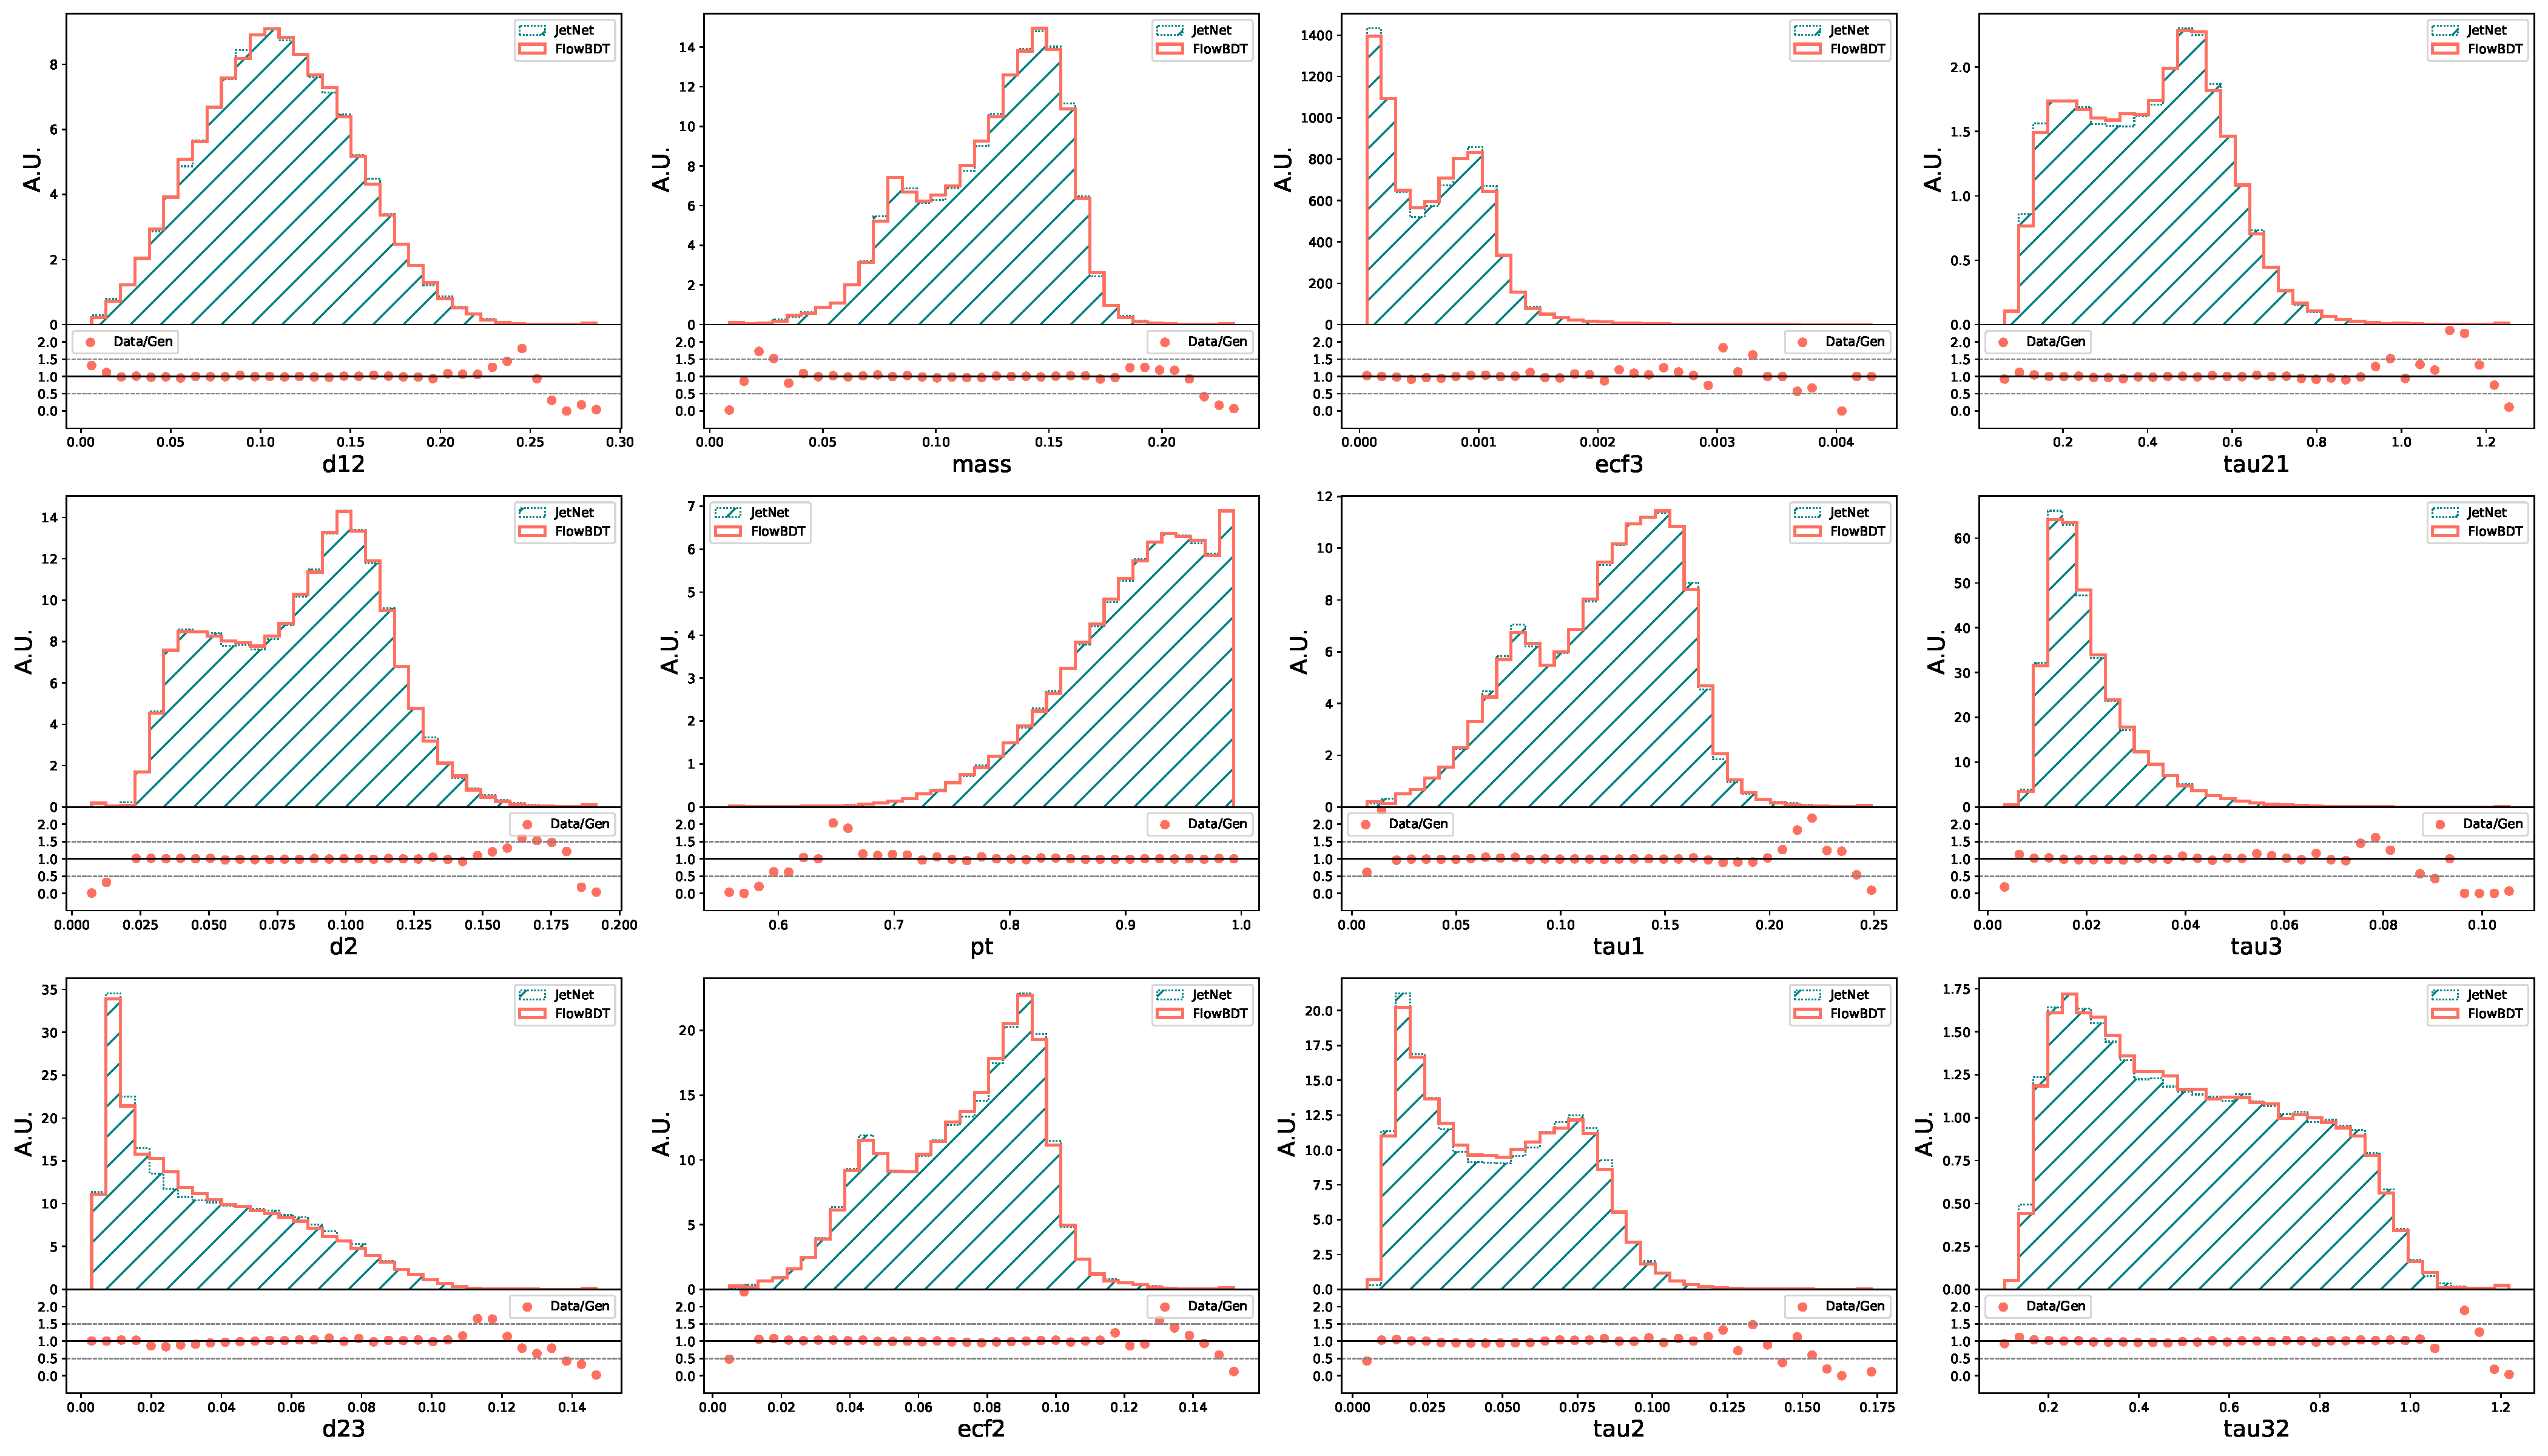
\includegraphics[width=\textwidth]{FLOWBDT/figures1/flowbdt_plot/jetnet.pdf}
    \caption{Histogram and ratio plots for the 12 high-level jet variables. Shaded bands: JetNet (target), solid lines: flowBDT (generated).}
    \label{fig1}
\end{figure*}


\section{Results}\label{sec4}

In this section, we present results for various HEP applications. Section~\ref{subsec4.1} demonstrates baseline performance for end-to-end fast simulation, as done with traditional normalizing flows \cite{flashsim}. Section~\ref{subsec4.2} extends the approach to much higher dimensions for hundreds of calorimeter voxels and jet constituents; the per-feature marginals are well reproduced, while limitations in capturing the joint distribution at the particle level are quantified and discussed. Section~\ref{subsec4.3} illustrates conditional generation for unfolding, and Section~\ref{subsec4.4} demonstrates Schr{\"o}dinger Bridge refinement for mapping between fast and full simulation distributions.

\subsection{End to end fast simulation}\label{subsec4.1}

Most high-level variables used at the analysis level are derived through a long simulation chain involving digitization and reconstruction. Having sufficient statistics for these variables is crucial for many analyses, yet deriving them from the generator level is computationally demanding. A promising approach is to directly generate these high-level observables, bypassing intermediate steps to significantly reduce simulation time.

Many analysis-level variables have complex, non-Gaussian distributions, and the generative model must learn to reproduce an $N$-dimensional distribution with intricate shapes and correlations. We study this by simulating four-vector, substructure, and energy correlation function variables of highly boosted top jets. A similar approach of generating high-level jet observables was studied in~\cite{Kansal}. The total number of 12 variables calculated from 3 subjets of pseudo-jets by \textit{JetNet} are considered, specifically, the transverse momentum and mass of the jet $p^\mathrm{T}$, $m$, the $N$-subjettiness~\cite{nsubjettiness1,nsubjettiness2} for exclusive $n$-jet $\tau_1$, $\tau_2$, $\tau_3$, the $N$-subjettiness ratios $\tau_{21} = \frac{\tau_2}{\tau_1}$, $\tau_{32} = \frac{\tau_3}{\tau_2}$, energy splitting functions defined by the splitting scale for $n$-jet exclusive clustering $d_{12}$, $d_{23}$, $n$\textsuperscript{th} order energy correlation functions~\cite{ecf} $ecf_2$, $ecf_3$ calculated from $p^\mathrm{T}$ and $\Delta R$, and finally $d_2 = \frac{ecf_3 \sum p^\mathrm{T}}{ecf_2^2}$. The input data has shape $(N, 12)$ where $N \approx 120\text{k}$ events.


The Dormand-Prince and Midpoint solvers with 20--30 steps already yield satisfactory results when generating 100k events for all variables. Fig.~\ref{fig1} shows that most variables with complex shapes exhibit good agreement between the target and generated distributions. The best histogram agreement is observed for substructure and splitting function variables related to the first two subjets, especially distributions with two asymmetric peaks. Despite a slight misalignment in the histograms of the third subjet, flowBDT performs well for tasks in the 10--20 dimensional regime with both low- and high-order ODE solvers.
\begin{figure*}[htbp]
    \centering
    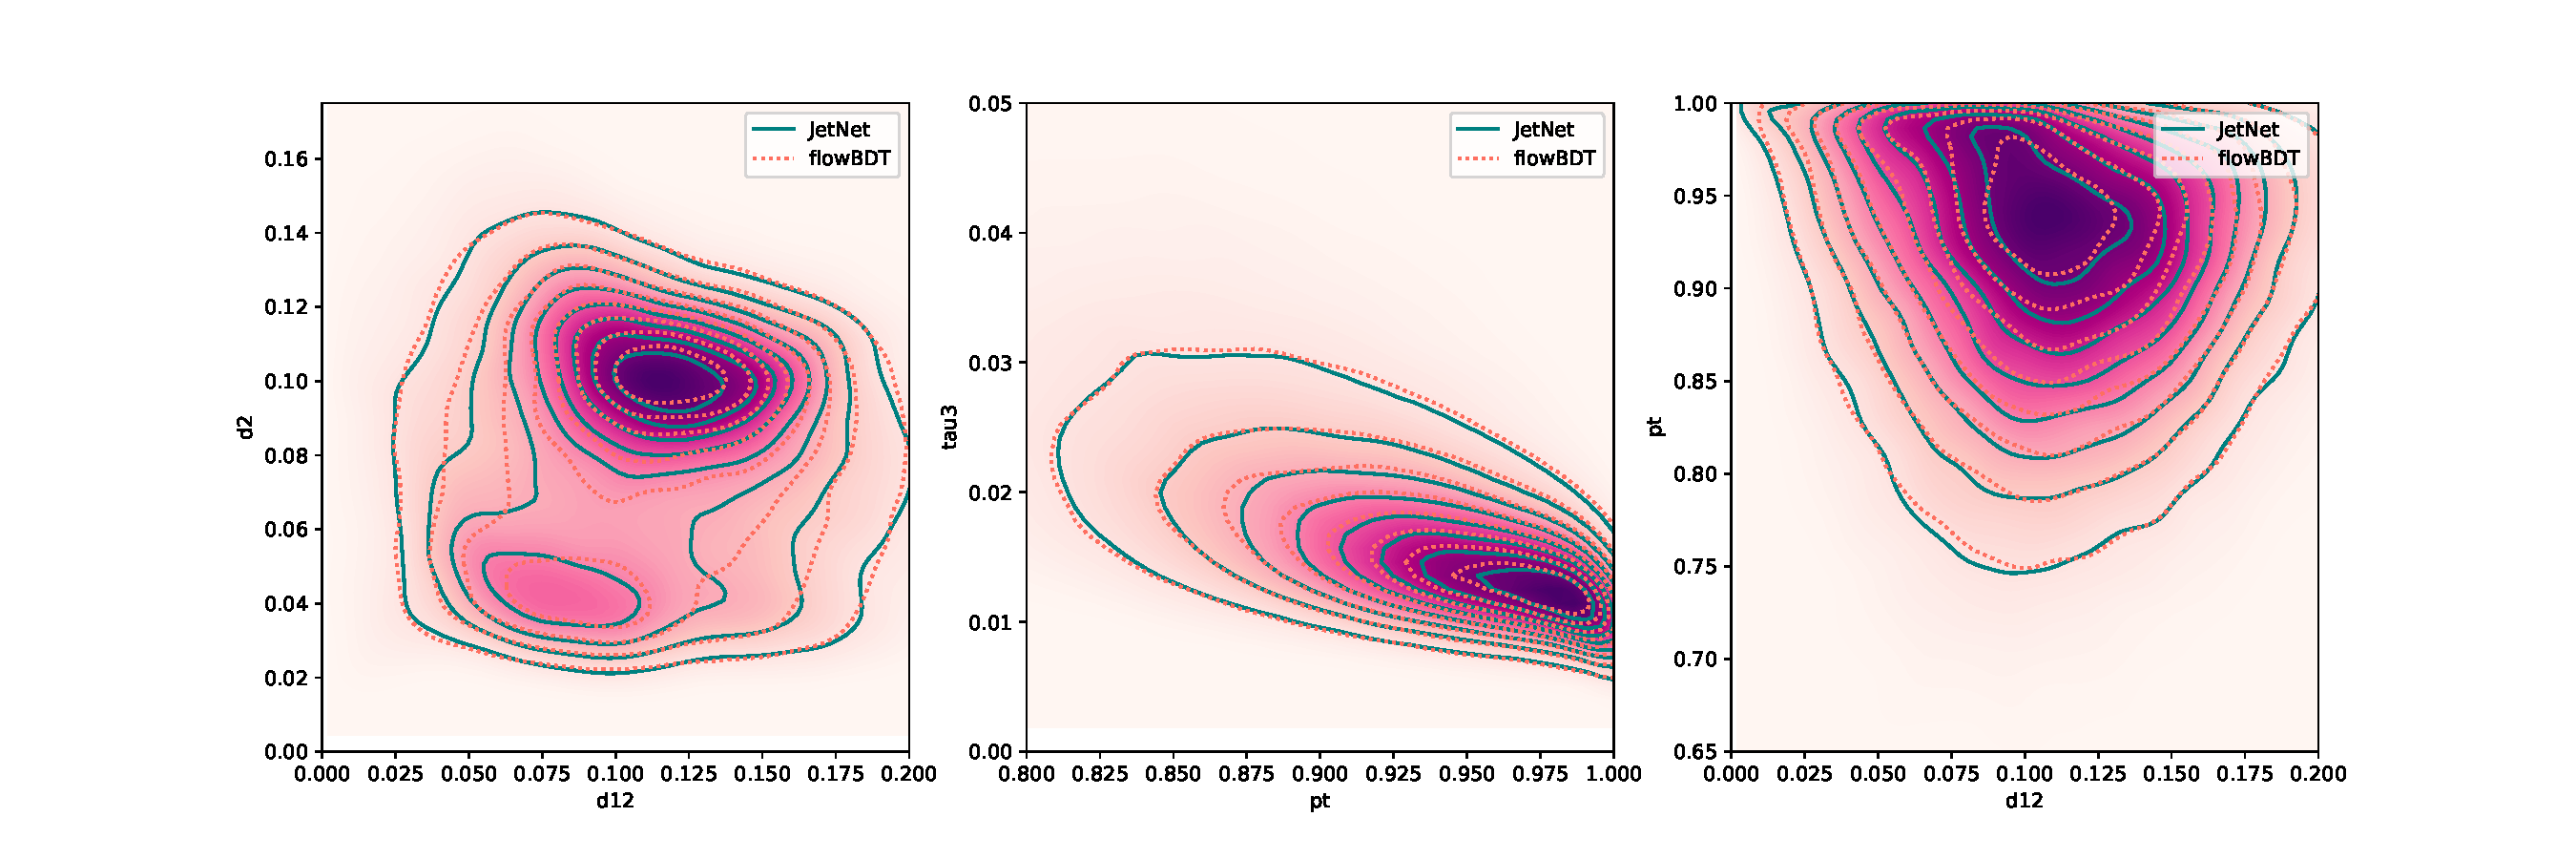
\includegraphics[width=\textwidth]{FLOWBDT/figures1/flowbdt_plot/contour_jn.pdf}
    \caption{Kernel density estimation contour plots for generated and original 100k jet variables. Solid lines: JetNet, dotted lines: flowBDT.}
    \label{fig2}
\end{figure*}

\begin{table}[htbp]
\begin{ruledtabular}
        \begin{tabular}{ccc}
        \textbf{Variable} & \textbf{Sep power}$\times 100$ & \textbf{W1}$\times 10$ \\
        \hline
        \textbf{$d_{12}$} & $0.147 \pm 0.013$ \,$(0.028 \pm 0.006)$ & $0.0066 \pm 0.0008$ \,$(0.0022 \pm 0.0007)$ \\
        \textbf{$d_{23}$} & $0.571 \pm 0.022$ \,$(0.026 \pm 0.005)$ & $0.0113 \pm 0.0004$ \,$(0.0012 \pm 0.0005)$ \\
        \textbf{$d_2$} & $0.269 \pm 0.015$ \,$(0.028 \pm 0.006)$ & $0.0109 \pm 0.0005$ \,$(0.0017 \pm 0.0007)$ \\
        \textbf{$\tau_{1}$} & $0.301 \pm 0.017$ \,$(0.028 \pm 0.005)$ & $0.0200 \pm 0.0007$ \,$(0.0026 \pm 0.0009)$ \\
        \textbf{$\tau_{2}$} & $0.737 \pm 0.024$ \,$(0.026 \pm 0.005)$ & $0.0218 \pm 0.0005$ \,$(0.0018 \pm 0.0008)$ \\
        \textbf{$\tau_{3}$} & $0.283 \pm 0.017$ \,$(0.026 \pm 0.005)$ & $0.0057 \pm 0.0002$ \,$(0.0007 \pm 0.0002)$ \\
        \textbf{$mass$} & $0.292 \pm 0.017$ \,$(0.029 \pm 0.005)$ & $0.0136 \pm 0.0006$ \,$(0.0018 \pm 0.0007)$ \\
        \textbf{$p^\mathrm{T}$} & $0.164 \pm 0.012$ \,$(0.027 \pm 0.005)$ & $0.0166 \pm 0.0012$ \,$(0.0037 \pm 0.0016)$ \\
        \textbf{$\tau_{21}$} & $0.303 \pm 0.016$ \,$(0.027 \pm 0.005)$ & $0.0671 \pm 0.0029$ \,$(0.0106 \pm 0.0046)$ \\
        \textbf{$\tau_{32}$} & $0.245 \pm 0.014$ \,$(0.027 \pm 0.006)$ & $0.0819 \pm 0.0051$ \,$(0.0137 \pm 0.0056)$ \\
        \textbf{$ecf_2$} & $0.510 \pm 0.022$ \,$(0.027 \pm 0.005)$ & $0.0133 \pm 0.0004$ \,$(0.0012 \pm 0.0005)$ \\
        \textbf{$ecf_3$} & $1.269 \pm 0.033$ \,$(0.025 \pm 0.005)$ & $0.0004 \pm 0.0000$ \,$(<\!0.001)$ \\
       \end{tabular}

     \caption{Evaluation metrics for samples generated from flowBDT on the 12-feature JetNet high-level representation. The separation power (triangular discriminator) is calculated from binned histograms; the Wasserstein-1 (W1) distance is computed on unbinned distributions. Uncertainties are obtained by bootstrap resampling ($n=100$). Numbers in parentheses are the corresponding truth-baseline floors, evaluated between two independent halves of the real data with the same bootstrap procedure, and indicate the resolution set by finite statistics. Both flowBDT and truth values are computed on the same evaluation run; older paper-era numbers are superseded by this self-consistent reanalysis.}
     \label{tab1}
\end{ruledtabular}
\end{table}


Quantitative evaluation metrics for binned and unbinned distributions are provided in Table~\ref{tab1}. Nearly all features sampled from the model yield low values of the triangular discriminator \cite{sep,tmva}, a specific $f$-divergence metric. The Wasserstein-1 distance (Earth Mover's Distance) \cite{emd0,wgan} also remains small for the majority of generated features. All metrics are reported with bootstrap uncertainties and compared against a finite-sample truth baseline, obtained by evaluating the metric on two independent halves of the real data, to establish the floor set by limited statistics. For a more comprehensive evaluation, variables simulated from the model should also exhibit correct pairwise correlations. Correlation contour plots, estimated using a Gaussian kernel, for representative variables ($d_{12}$, $p^\mathrm{T}$, $\tau_3$) are shown in Fig.~\ref{fig2}. We find the model reproduces the same shape on every level of the contour lines, even for plots with multiple peak rings. As an additional consistency check, we compare the directly generated $\tau_{21}$ (and $\tau_{32}$) with the ratios computed from the independently generated $\tau_1$, $\tau_2$ (and $\tau_3$). The Wasserstein-1 distances between the two are $\sim 0.014$ for $\tau_{21}$ and $\sim 0.029$ for $\tau_{32}$, confirming that the model learns the correct inter-variable correlations to within finite-sample resolution. As a stronger joint test, we additionally train an MLP-based classifier to distinguish real from generated samples on the 12-feature representation; the resulting AUC is $0.9994 \pm 0.0002$ (bootstrap, $n=20$). For reference, the same MLP architecture applied to two independent random halves of the real data yields AUC $= 0.498 \pm 0.002$ (mean and standard deviation over five splits), confirming that the discriminator is calibrated at chance and that the near-unity AUC against flowBDT reflects a genuine distributional gap rather than finite-sample overfitting by the classifier. The near-perfect AUC reflects the limitation of the per-feature regression strategy in fully capturing higher-order joint correlations, together with min-max boundary-clipping artefacts that arise when generated values saturate at the training-range edges.

As demonstrated above, flowBDT generates samples of high quality with negligible inference time of 0.4--0.8\,ms per event. Training is also fast for low-dimensional tasks: using small BDT trees trained independently per time step on a single CPU thread, the training time for 120k events is approximately 3--4 minutes per core.

\subsection{Low level simulation for cells and jet constituents}\label{subsec4.2}

To fully explore the potential of our model, we increase the dimension of the input features to the next magnitude. In this study, we focus on dataset~1 which contains layers with different granularities. There are ways to map the features into a latent space, or treat them as a flattened array to deal with irregular geometry. The latter does not treat the shower as 3-D or structured data. Following this logic, all the voxel energies are treated as tabular data with shape $(N, 368)$ for dataset~1 and $(N, 90)$ for the JetNet particle-level data (30 particles $\times$ 3 features).

By default, each GBT regression model produces a single output of shape $(N,1)$, so the number of voxels per shower determines the number of GBT models required per time step. Instead, we employ a multi-output tree strategy where each tree produces one output per feature, reducing the total to a single GBT model per time step. This yields a 5--8$\times$ speedup during inference with indistinguishable performance.
\begin{figure*}[htbp]
    \centering
    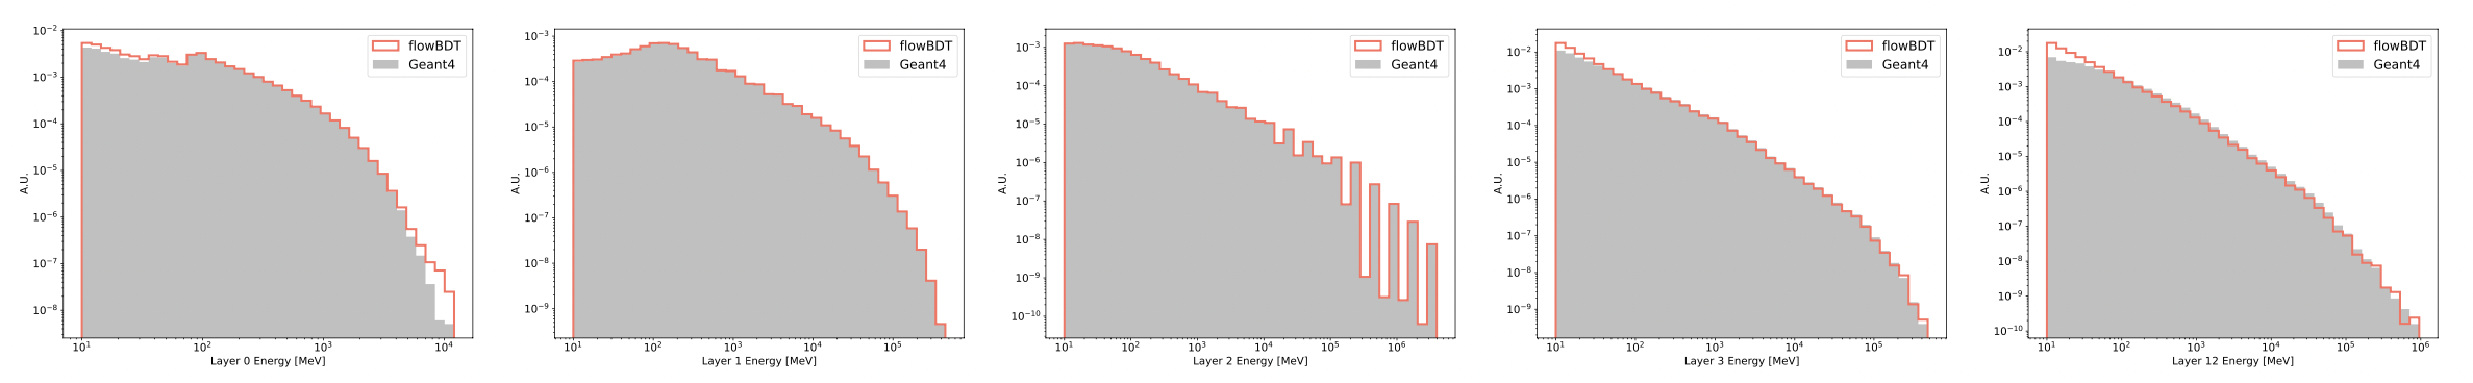
\includegraphics[width=\textwidth]{FLOWBDT/figures1/flowbdt_plot/elayer.pdf}
    \caption{Different calorimeter layer energies of the photon sample generated by flowBDT and Geant4.}
    \label{fig3}
\end{figure*}

In Fig.~\ref{fig3}, the raw voxel outputs are summed according to the $\alpha$ and $r$ bins of each layer. flowBDT predicts well for the more granular layers~1 and~2. However, a shortfall becomes apparent in the energy distribution tails of layer~0 and for showers with low energy deposited in the last layer.

\begin{figure}[htbp]
    \centering
        \centering
        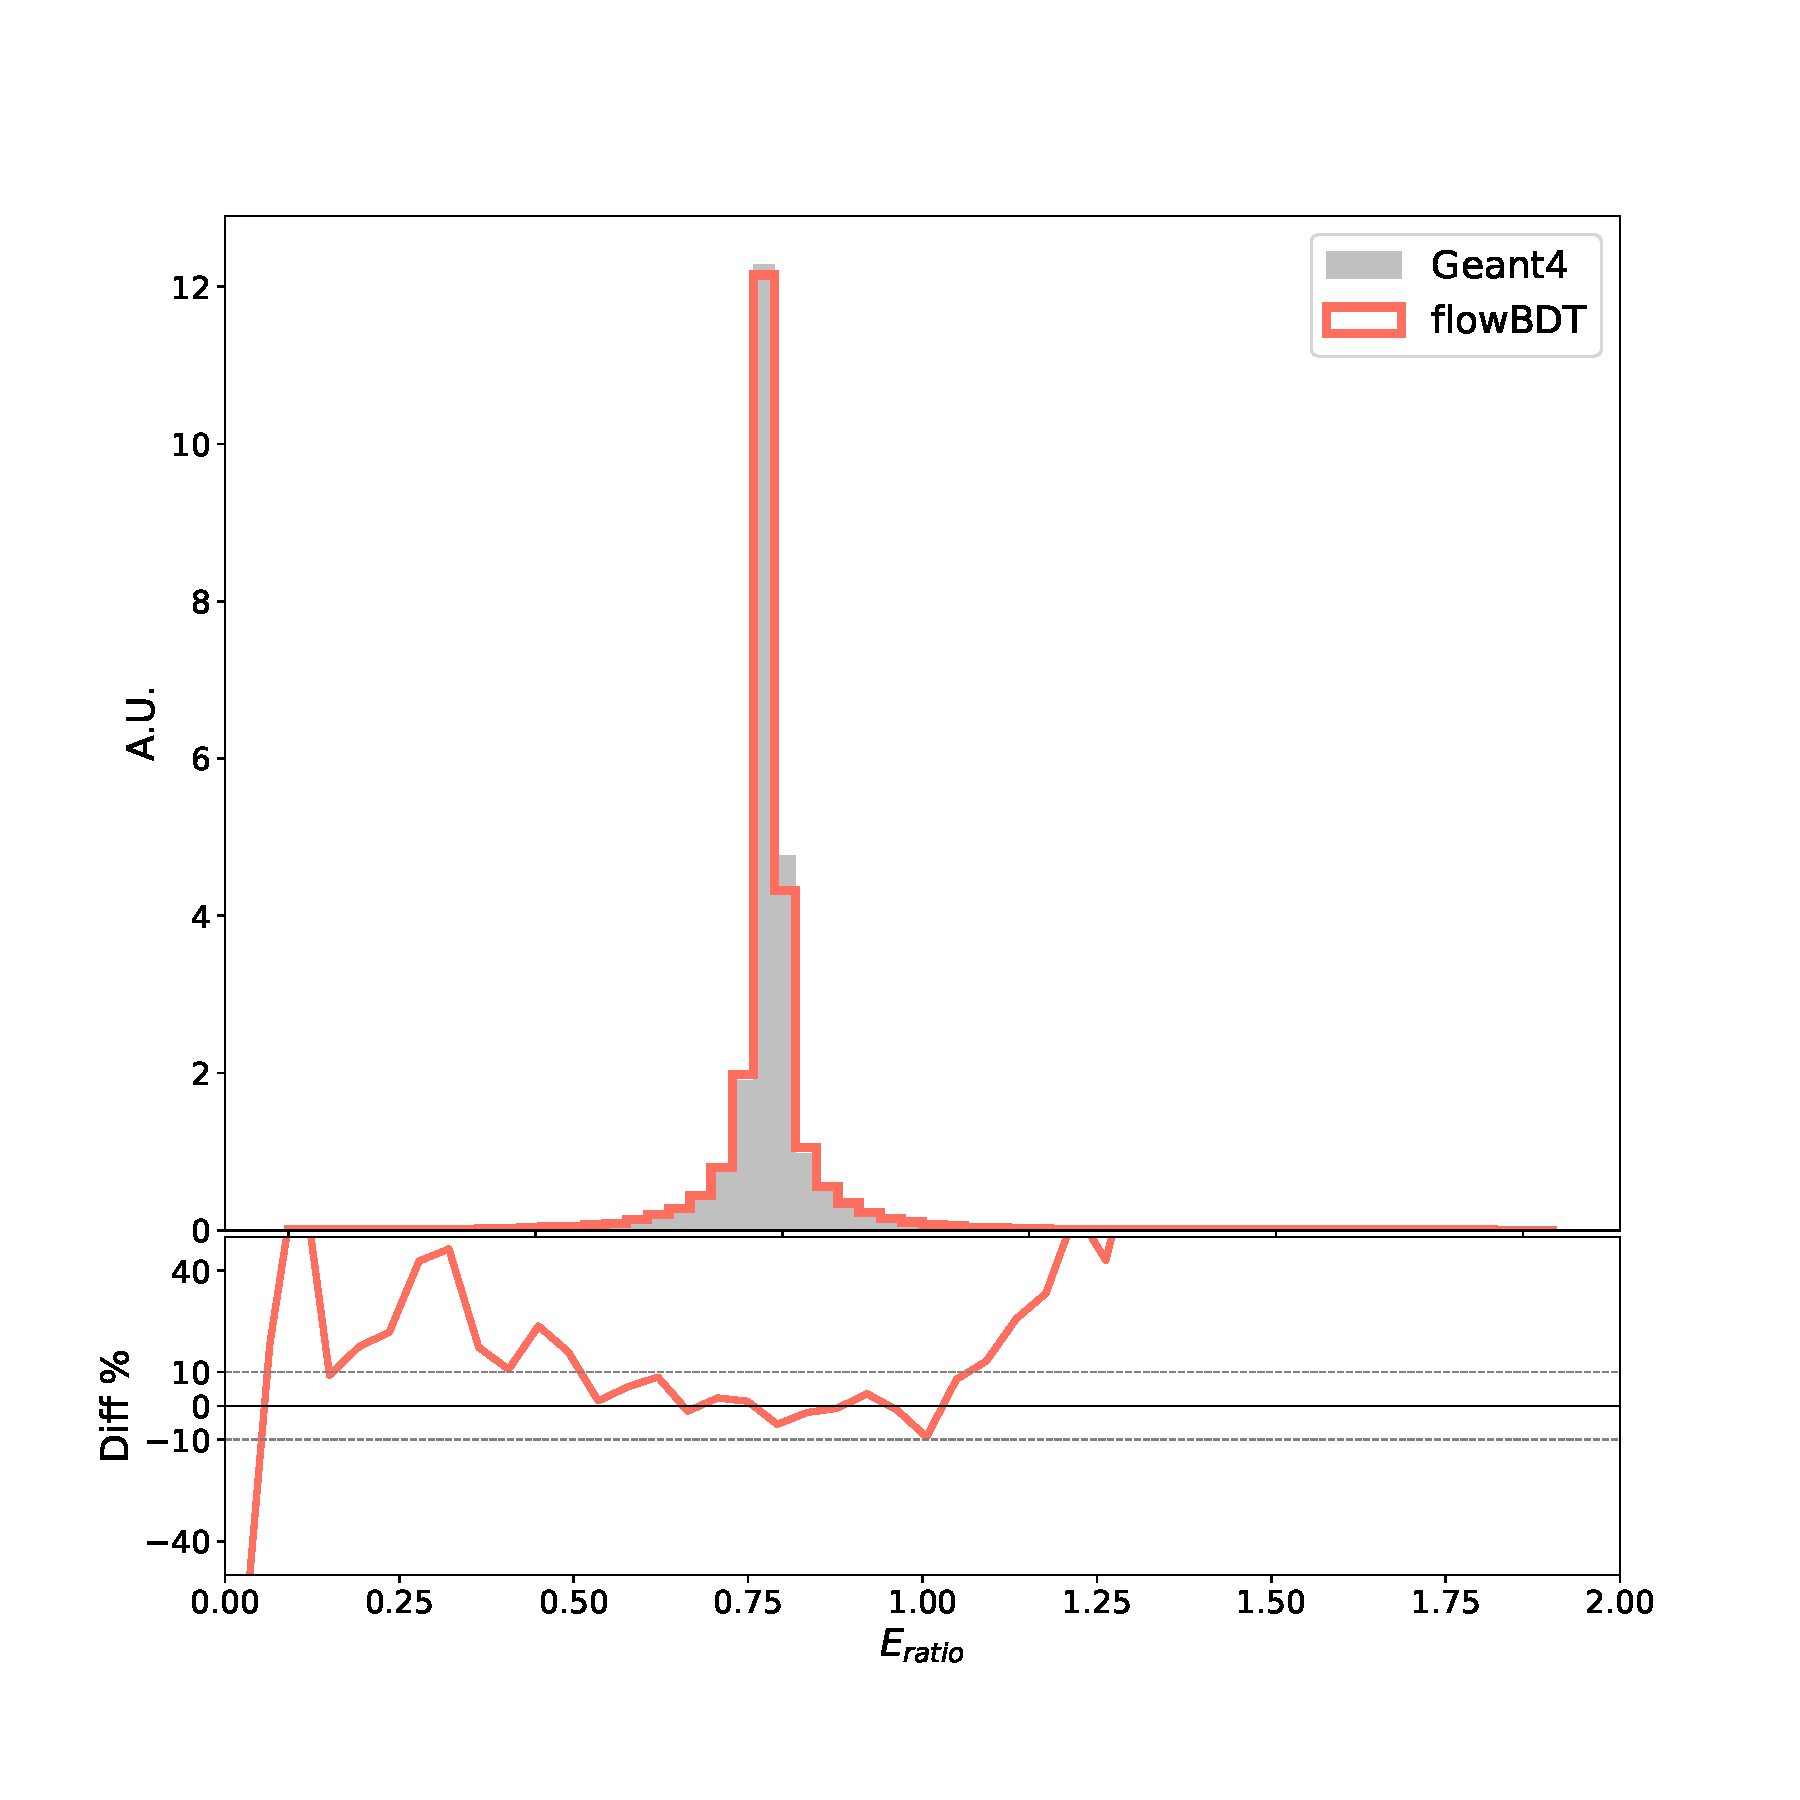
\includegraphics[width=0.6\linewidth]{FLOWBDT/figures1/flowbdt_plot/shower_response_low-1.pdf}
        \caption{Shower response histogram and ratio plot of the photon sample generated by flowBDT and Geant4.}\label{fig4}
    
\end{figure}

Shower response $E_{ratio}$ as an important quantity used in calibrating objects is shown in Fig.~\ref{fig4}. The $E_{ratio}$ generated by the model exhibits a shape and peak width closely mirroring those produced by Geant4. A similar correspondence is observed for another variable concerning the shower location, the center of energy in the $\eta$ and $\phi$ directions: $\Bar{\eta} = \frac{\langle \eta_i E_i \rangle}{\sum E_i}$ for cell location $\eta_i$, as illustrated in Figure~\ref{fig5}.
\begin{figure}[htbp]
    \centering
        \centering
        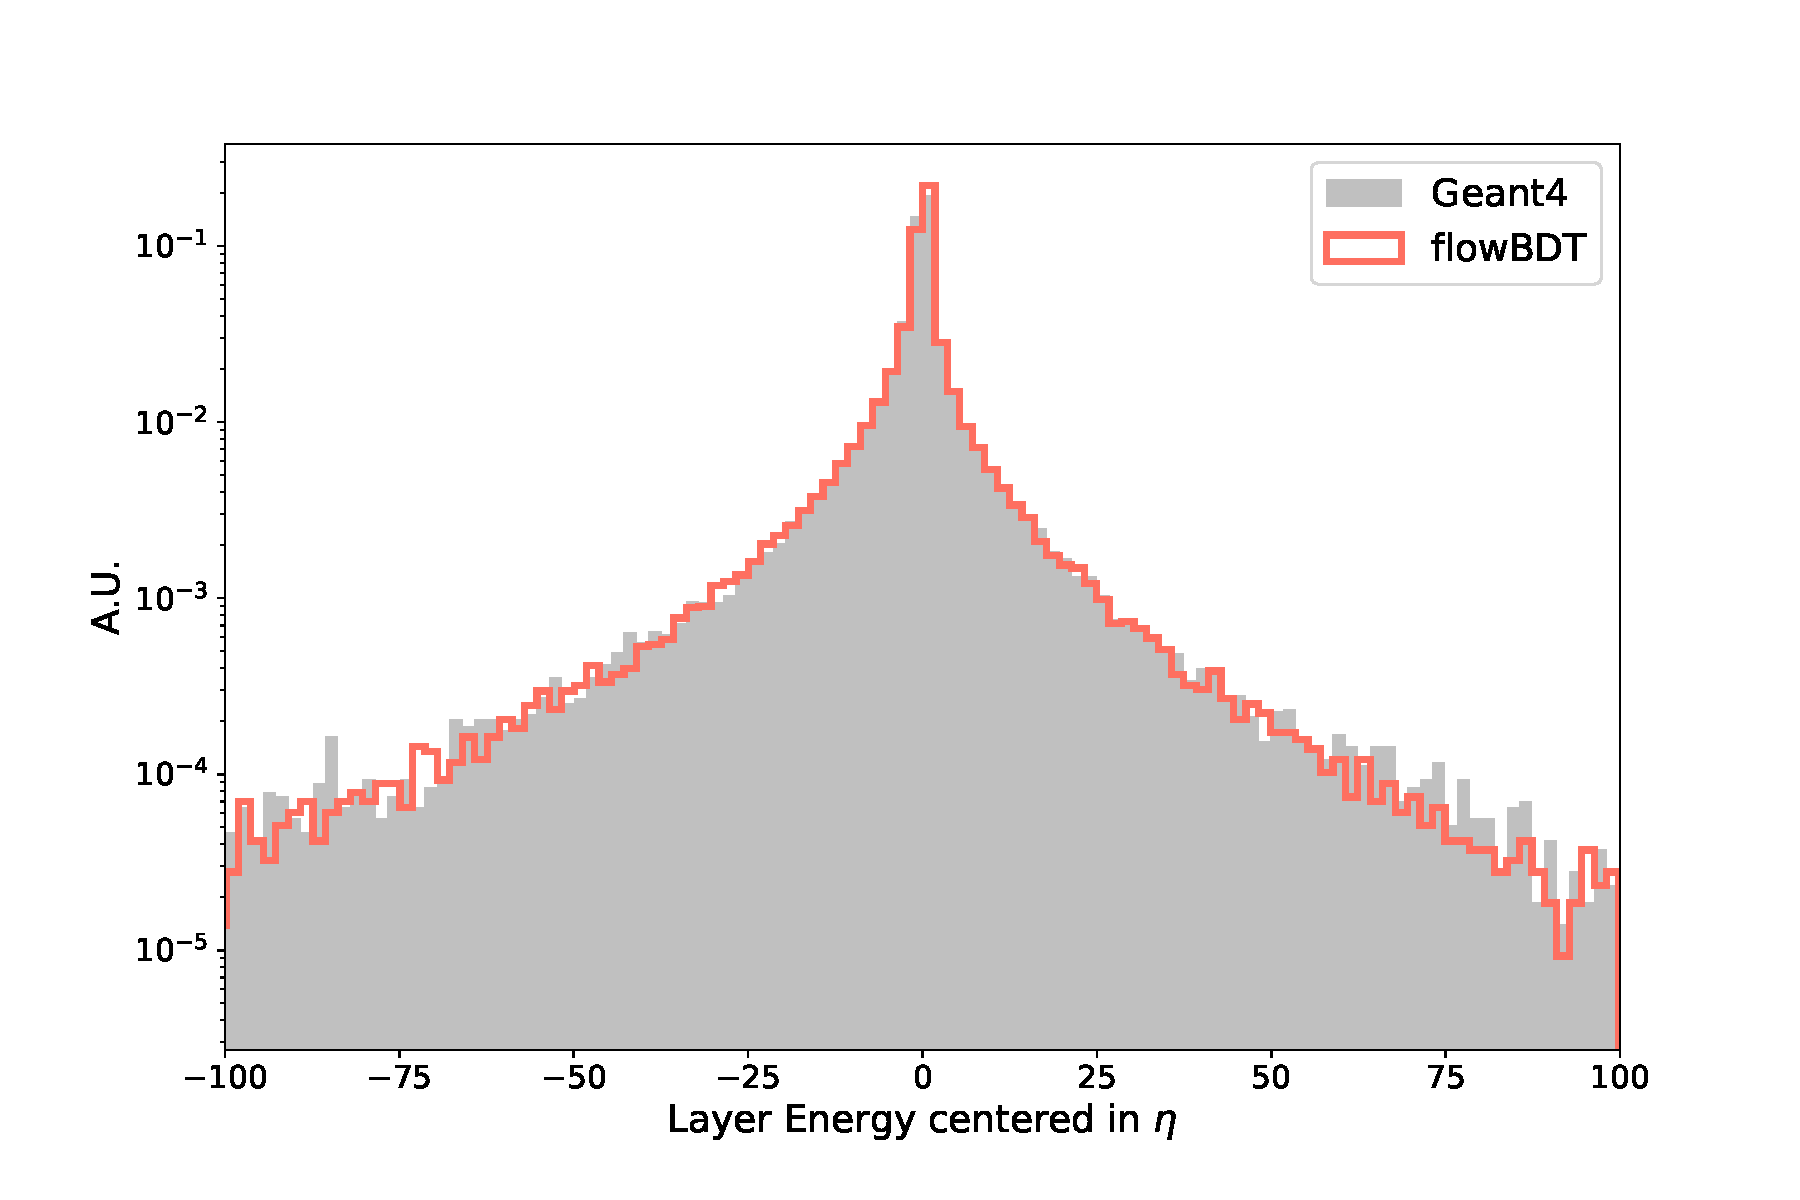
\includegraphics[width=0.45\linewidth]{FLOWBDT/figures1/flowbdt_plot/energyeta_low.pdf} \quad
        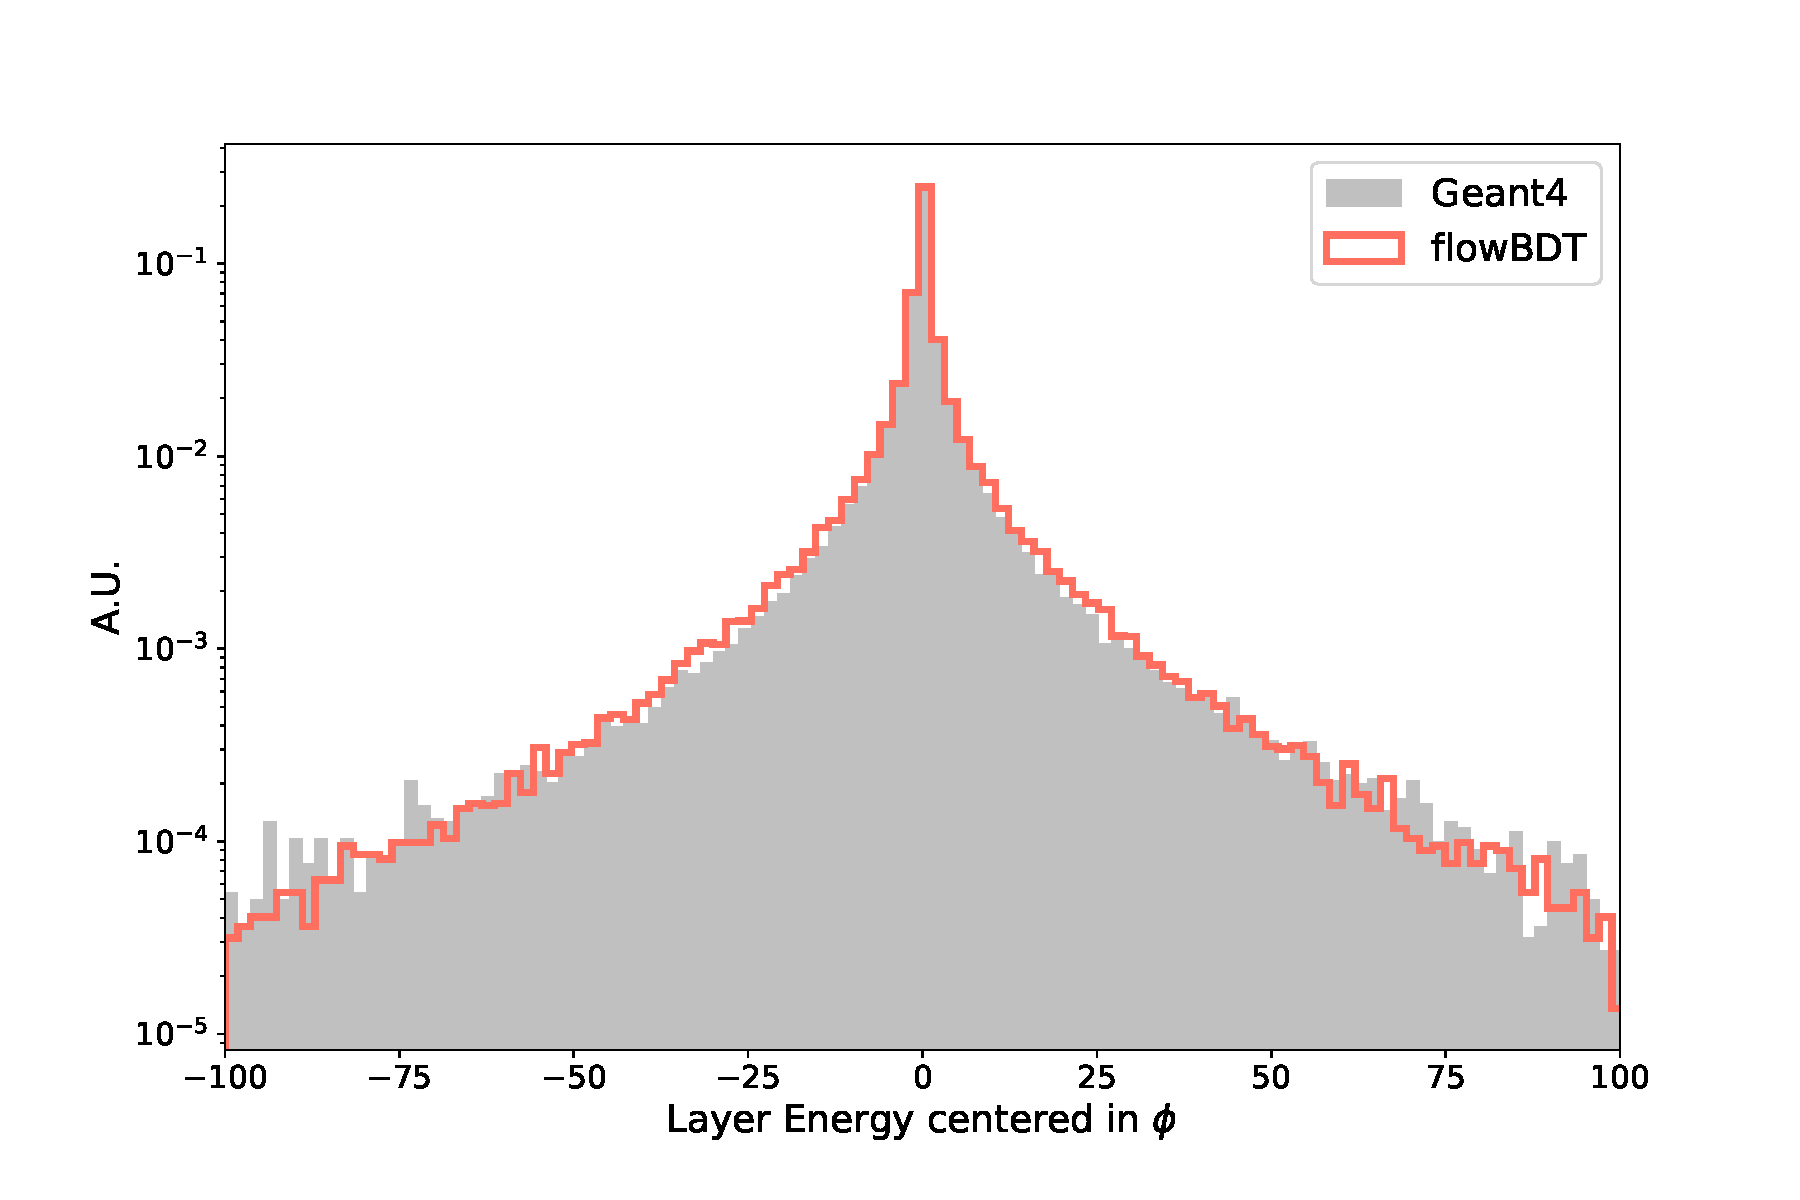
\includegraphics[width=0.45\linewidth]{FLOWBDT/figures1/flowbdt_plot/energyphi_low.pdf}
        \caption{Center of energy in $\eta$ and $\phi$ direction on second layer of the photon shower generated by flowBDT and Geant4}\label{fig5}

\end{figure}

To complement the marginal-distribution checks above, we additionally train an MLP-based classifier to distinguish real Geant4 from generated flowBDT samples on an 8-feature high-level representation (energy response, five layer fractions, shower depth and width). The bootstrap-averaged AUC is $0.9995 \pm 0.0002$, with the corresponding ROC curve shown in Fig.~\ref{fig:calo_roc}. As in the JetNet case, the near-unity AUC reflects the per-feature regression's inability to enforce exact joint correlations together with min-max boundary-clipping artefacts at the training-range edges, rather than gross failure of the marginal distributions.

\begin{figure}[htbp]
    \centering
        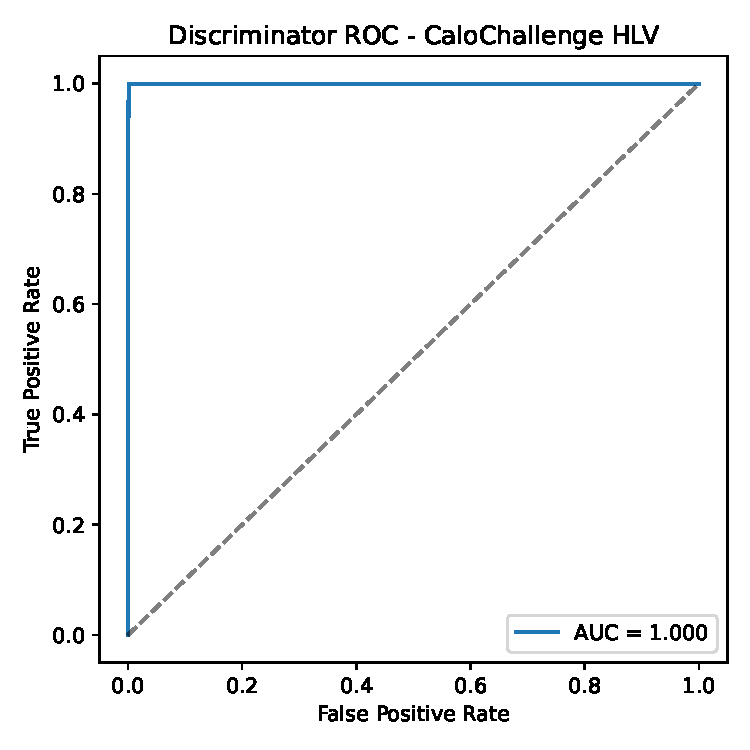
\includegraphics[width=0.6\linewidth]{FLOWBDT/figures1/flowbdt_plot/calo_roc_curve.pdf}
        \caption{ROC curve of the MLP classifier trained to distinguish real Geant4 photon showers from those generated by flowBDT, evaluated on the 8-feature CaloChallenge high-level representation. The bootstrap-averaged AUC is $0.9995 \pm 0.0002$.}\label{fig:calo_roc}
\end{figure}

\begin{figure*}[htbp]
    \centering

    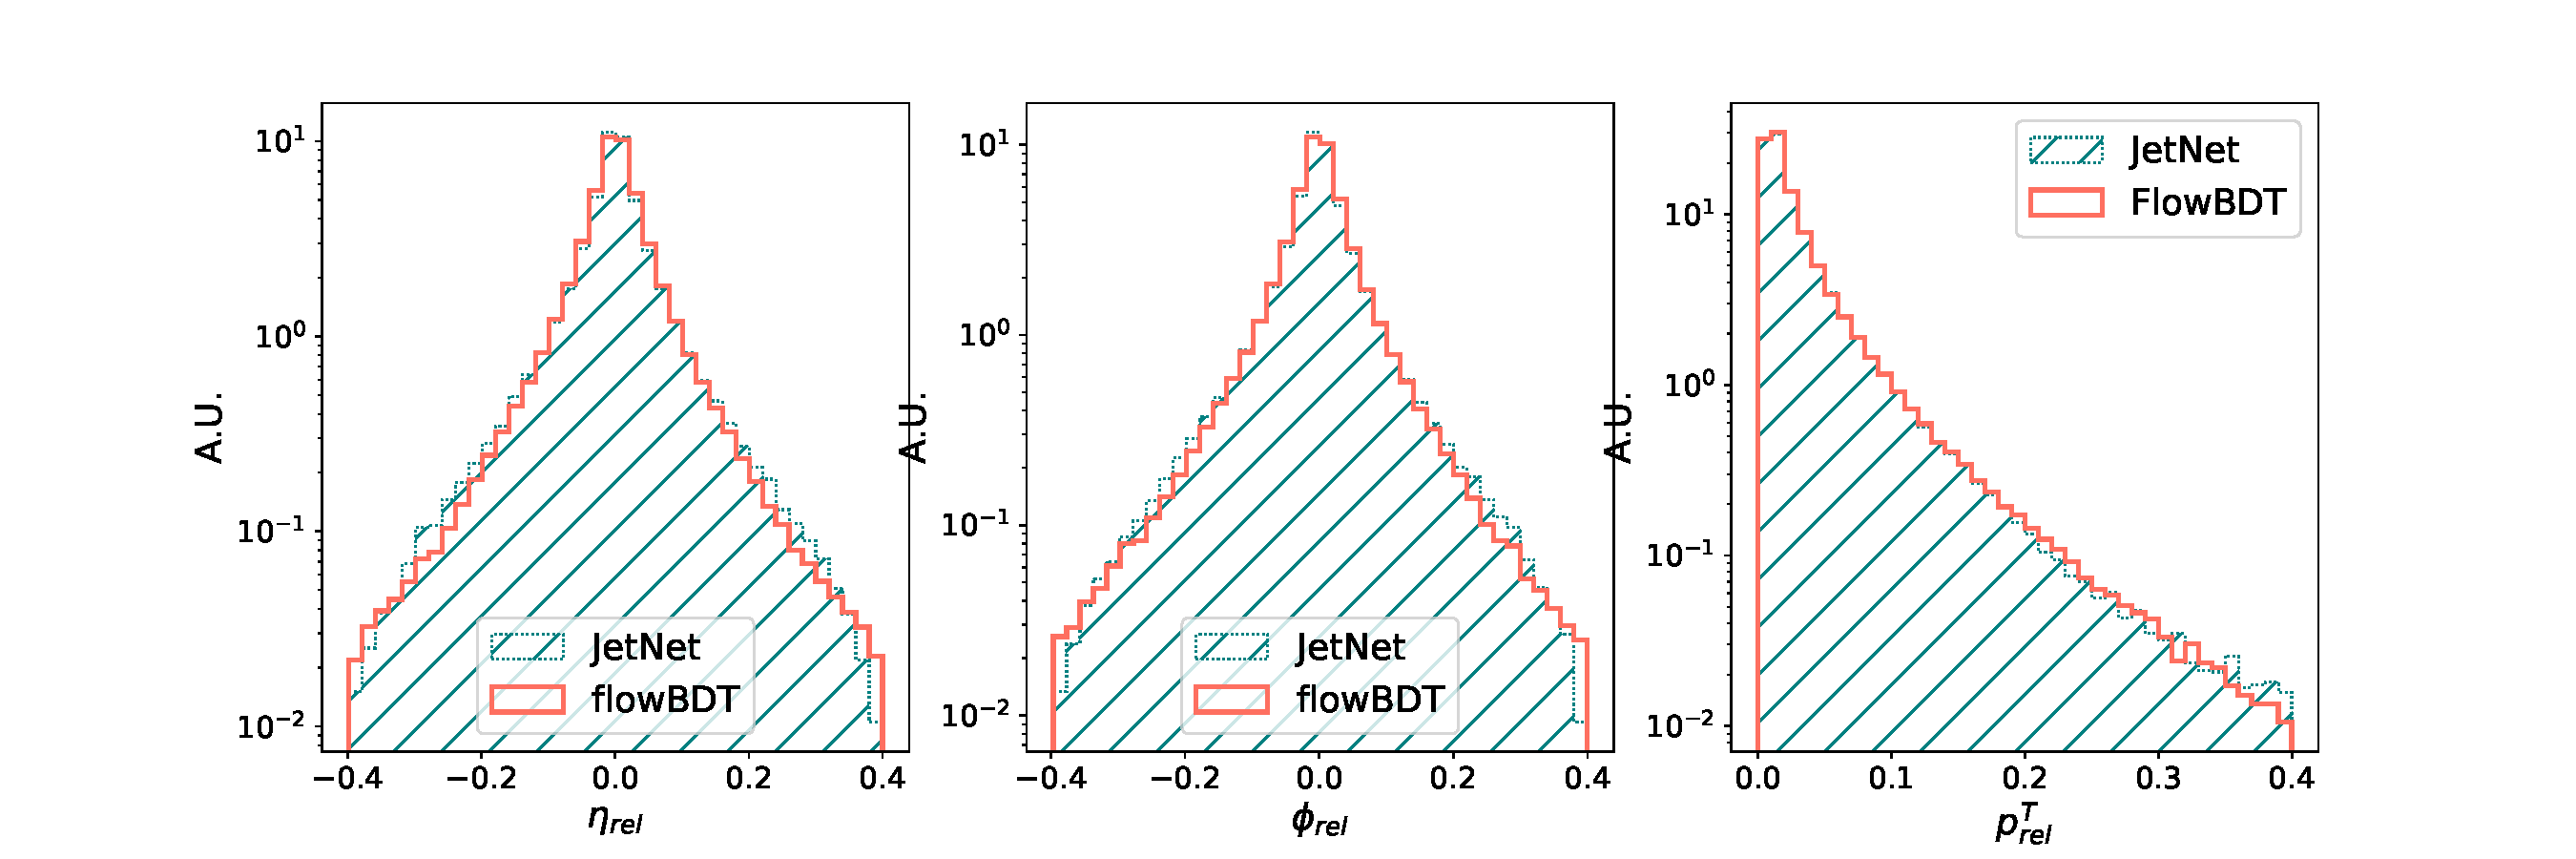
\includegraphics[width=\textwidth]{FLOWBDT/figures1/flowbdt_plot/jn_high.pdf}
    \caption{Relative location and $p^\mathrm{T}$ of the jet constituents inside gluon-initiated jets from flowBDT and JetNet.} 
    \label{fig6}
\end{figure*}

\begin{figure*}[htbp]
    \centering

    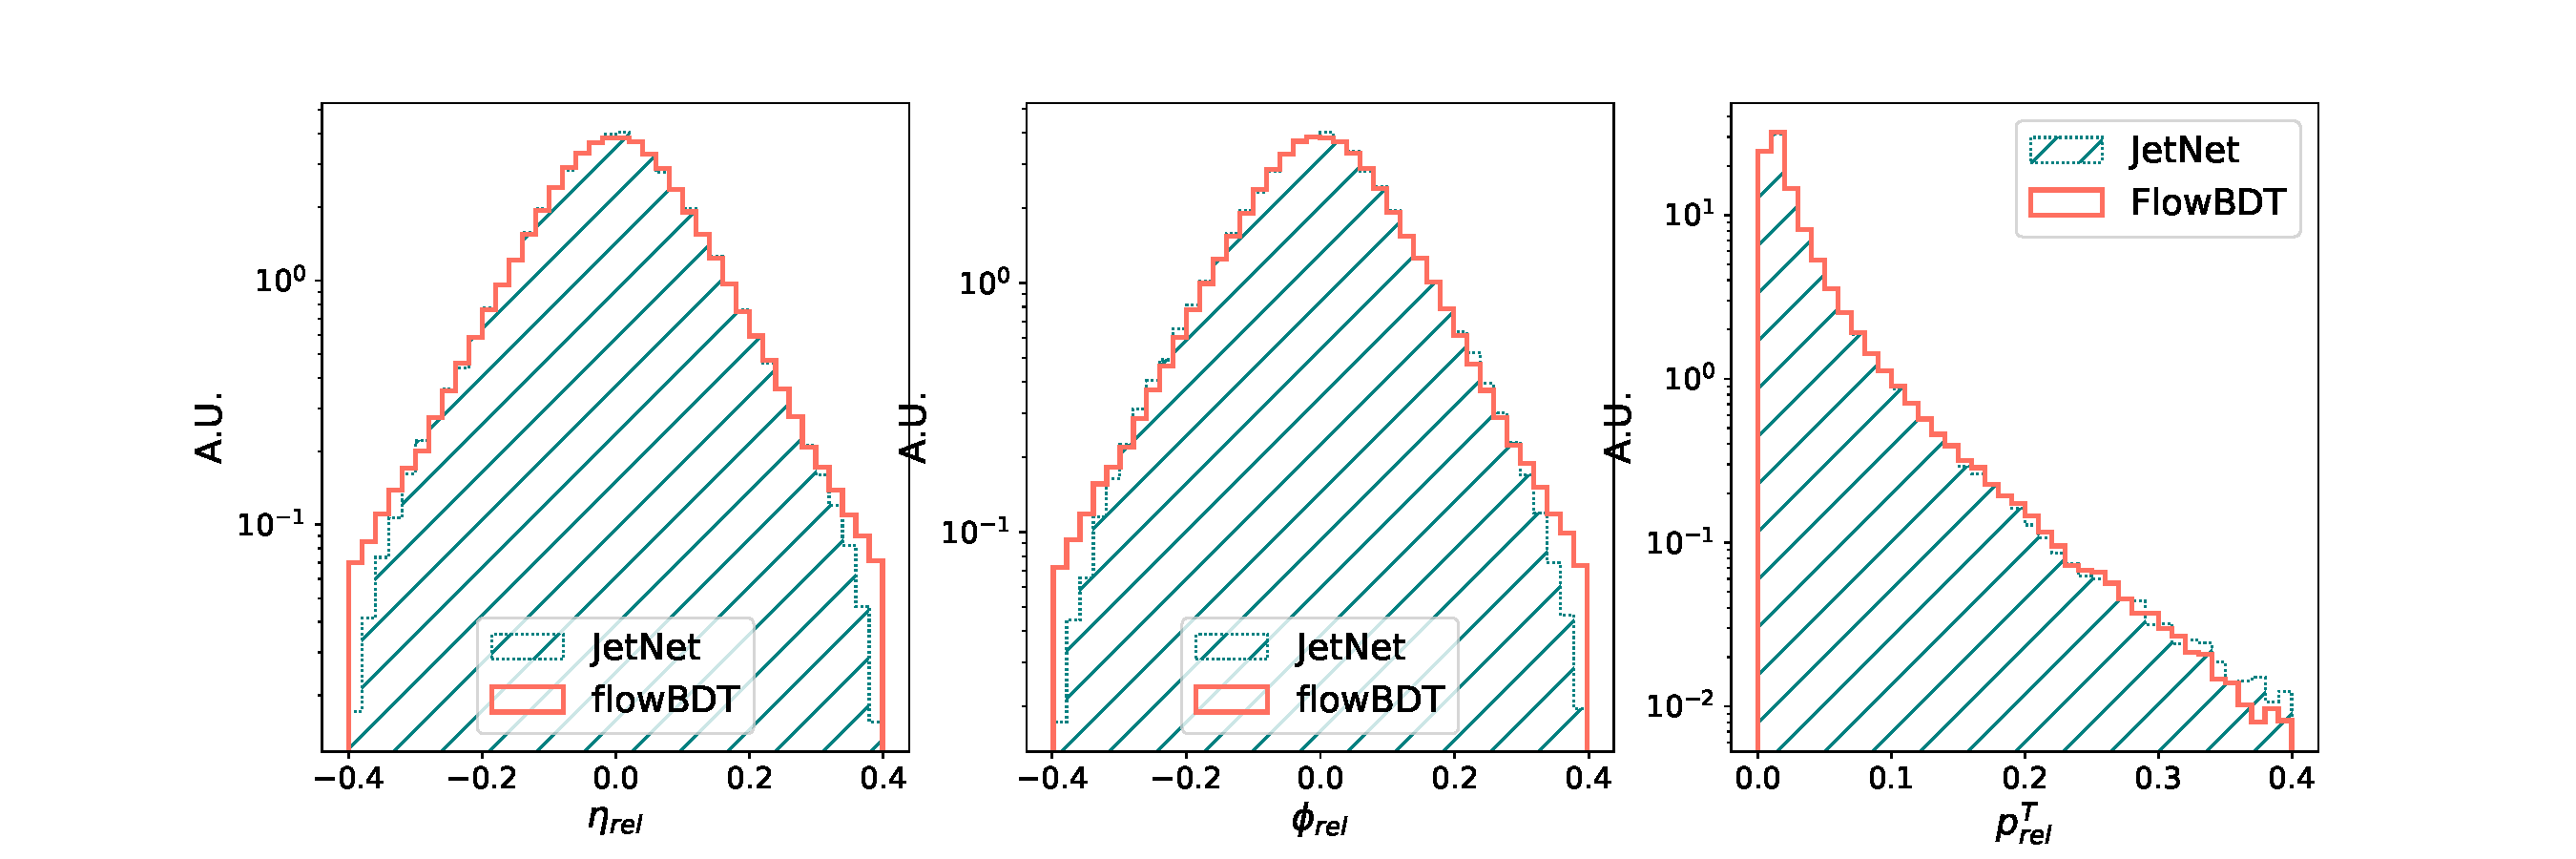
\includegraphics[width=\textwidth]{FLOWBDT/figures1/flowbdt_plot/jn_high_top.pdf}
    \caption{Relative location and $p^\mathrm{T}$ of the jet constituents inside top quark jets from flowBDT and JetNet.} 
    \label{fig7}
\end{figure*}



The same treatment is applied to the JetNet dataset, where the goal is to regress the raw particle-level four-vector data for gluon-initiated and top jets. The generated relative $p^\mathrm{T}$ distribution shows reasonable alignment with the target at the level of individual particles, but visible deficiencies appear in the tails of the relative angular distributions, as illustrated in Figure~\ref{fig7}. Following the JetNet benchmark of Ref.~\cite{Kansal}, we additionally report unbinned Wasserstein-1 metrics in Table~\ref{tab2}: the W1 distance on the jet mass (derived from the 30~constituents via the standard massless--particle relation), on the jet relative $p_T$ (a sanity check, since $\sum_i p_T^{\mathrm{rel},i}\!\simeq\!1$ by construction), and on each of the three per-particle distributions ($\eta^\mathrm{rel}$, $\phi^\mathrm{rel}$, $p_T^\mathrm{rel}$) flattened across all particles. Two columns are reported: ``Raw'' is the unmodified generator output, and ``+ pt renorm'' applies a per-jet post-hoc rescaling so that the generated $\sum_i p_T^{\mathrm{rel},i}$ matches a sample drawn from the empirical real-data distribution. The per-particle marginals lie within a factor of $\sim\!50$ of the truth floor, and the post-hoc rescaling brings W1-Pt down to a comparable level; however, the per-particle angular distributions and the jet mass remain three orders of magnitude above the floor in both columns. This contrast highlights the central limitation of per-feature regression in this regime: each of the $30 \times 3$ outputs is modelled independently with a multi-output tree backbone, but the regression objective is per-feature MSE and so does not directly constrain the angular structure that determines $m_\mathrm{jet}$. A model with an explicit jet--level loss (e.g.\ adding a $W_1(m_\mathrm{jet})$ regularizer or a Soft Drop--style auxiliary objective) would be required to close this gap; we flag it as future work in Sec.~\ref{sec5}.

\begin{table}[htbp]
\begin{ruledtabular}
        \begin{tabular}{lccc}
        \textbf{Variable} & \textbf{Metric} & \textbf{Raw} & \textbf{+ pt renorm} \\
        \hline
        $m_\mathrm{jet}/p_T^\mathrm{jet}$            & W1-M  & $242.16 \pm 0.21$ & $183.66 \pm 0.14$ \\
        $p_T^\mathrm{jet}/p_T^\mathrm{jet}$ (sanity) & W1-Pt & $198.68 \pm 0.65$ & $17.25 \pm 0.22$ \\
        per-particle $\eta^\mathrm{rel}$             & W1-P($\eta$)   & $166.35 \pm 0.58$ & $164.76 \pm 0.48$ \\
        per-particle $\phi^\mathrm{rel}$             & W1-P($\phi$)   & $113.60 \pm 0.40$ & $113.11 \pm 0.44$ \\
        per-particle $p_T^\mathrm{rel}$              & W1-P($p_T$)    & $9.07 \pm 0.20$ & $4.97 \pm 0.11$ \\
        \hline
        truth-baseline floor                         &       & \multicolumn{2}{c}{$\{0.18 / 0.38 / 0.70 / 0.70 / 0.24\}$} \\
        \end{tabular}
     \caption{Particle-level JetNet 30$\times$3 evaluation (W1 $\times 10^3$): Wasserstein-1 distances between flowBDT-generated and real top-jet samples for the derived jet observables (W1-M, W1-Pt) and for each per-particle feature (W1-P), following the benchmark of Ref.~\cite{Kansal}. Generator hyper-parameters: multi-output XGBoost, max\_depth$=6$, n\_estimators$=200$, $\eta=0.05$, duplicate-$K=20$, 30 timesteps with the DOPRI5 solver (30 steps). Uncertainties are obtained by bootstrap resampling ($n=100$). The ``Raw'' column reports the unmodified generator output; the ``+ pt renorm'' column applies a per-jet post-hoc rescaling so that $\sum_i p_T^{\mathrm{rel},i}$ matches a sample drawn from the empirical real-data distribution. Truth-baseline floors are obtained between two independent halves of the real data with the same bootstrap procedure, listed in the same row order. The post-hoc rescaling collapses W1-Pt and W1-P($p_T$) to a single-digit factor of $\sim\!50\times$ the floor; however, the per-particle angular distributions and the jet mass remain two-to-three orders of magnitude above the floor, because per-feature regression treats each of the $30\times3$ outputs independently and does not preserve the angular structure that determines $m_\mathrm{jet}$. Closing this remaining gap requires a backbone with an explicit jet-level objective (Sec.~\ref{sec5}).}
     \label{tab2}
\end{ruledtabular}
\end{table}



\subsection{Unfolding via conditional generation}\label{subsec4.3}

Due to the restricted resolution and acceptance of detectors, the distributions of detector-level quantities diverge from those at the particle level. One important technique used in collider physics is unfolding, which corrects these detector effects. Machine learning-based unfolding methods \cite{cinnfold,sbfold,omnifold} offer significant advantages for unbinned and high-dimensional differential cross-section measurements. Most generative models encounter similar challenges when attempting to generate high-quality samples from non-Gaussian priors in large dimensions or from distributions that are significantly different from the target distribution. In this section, we show how conditional generation is tackled by the model in both low and high dimensions.

Using the public jet dataset~\cite{omnifold,omnifold_zenodo} with several MC generator/tune pairs, we consider the leading jet width and mass, multiplicity, $N$-subjettiness ratio between leading and subleading jets $\tau_{21} = \frac{\tau_2}{\tau_1}$, the normalized groomed mass $\ln\rho = \frac{\ln m_{SD}^2}{p_T^2}$ and momentum fraction $z_g$ for the Soft Drop grooming algorithm with specific angularity and cut \cite{softdrop0,softdrop1}. To assess the performance of the conditioned generation, we compare with the histograms generated from a Gaussian prior using both binned and unbinned metrics. As shown in Table~\ref{table1}, we find that the separation power and Wasserstein-1 distance from the non-Gaussian prior demonstrate better performance for the majority of observables. Fig.~\ref{fig8} shows the comparison histograms for the six unfolding observables. We denote samples generated from a Gaussian prior as ``Flow-Diffu'' and those generated from the reconstructed-level (conditioned) prior as ``Flow-OT'', following the notation of optimal transport conditional flow matching. More importantly, starting from a reconstructed level prior provides substantial benefits, as it captures the correlation of the target observables much more effectively than a multidimensional Gaussian would. If we define a relative improvement on correlation difference to be ratio of the sum of absolute values of those differences with data between simulation and generated sample:
\begin{gather}
    \mathcal{I}_{rel} = \frac{\sum_{i=1}^n Corr_{data,i}-Corr_{sim,i}}{\sum_{i=1}^n Corr_{data,i}-Corr_{gen,i}}
\end{gather}
The relative improvement for conditional generation is approximately 3040\%, significantly exceeding the 414\% improvement from the unconditional case. Both scenarios nevertheless show a substantial enhancement in overall correlation, as shown in Fig.~\ref{fig9}.


\begin{figure*}[htbp]
    \centering
    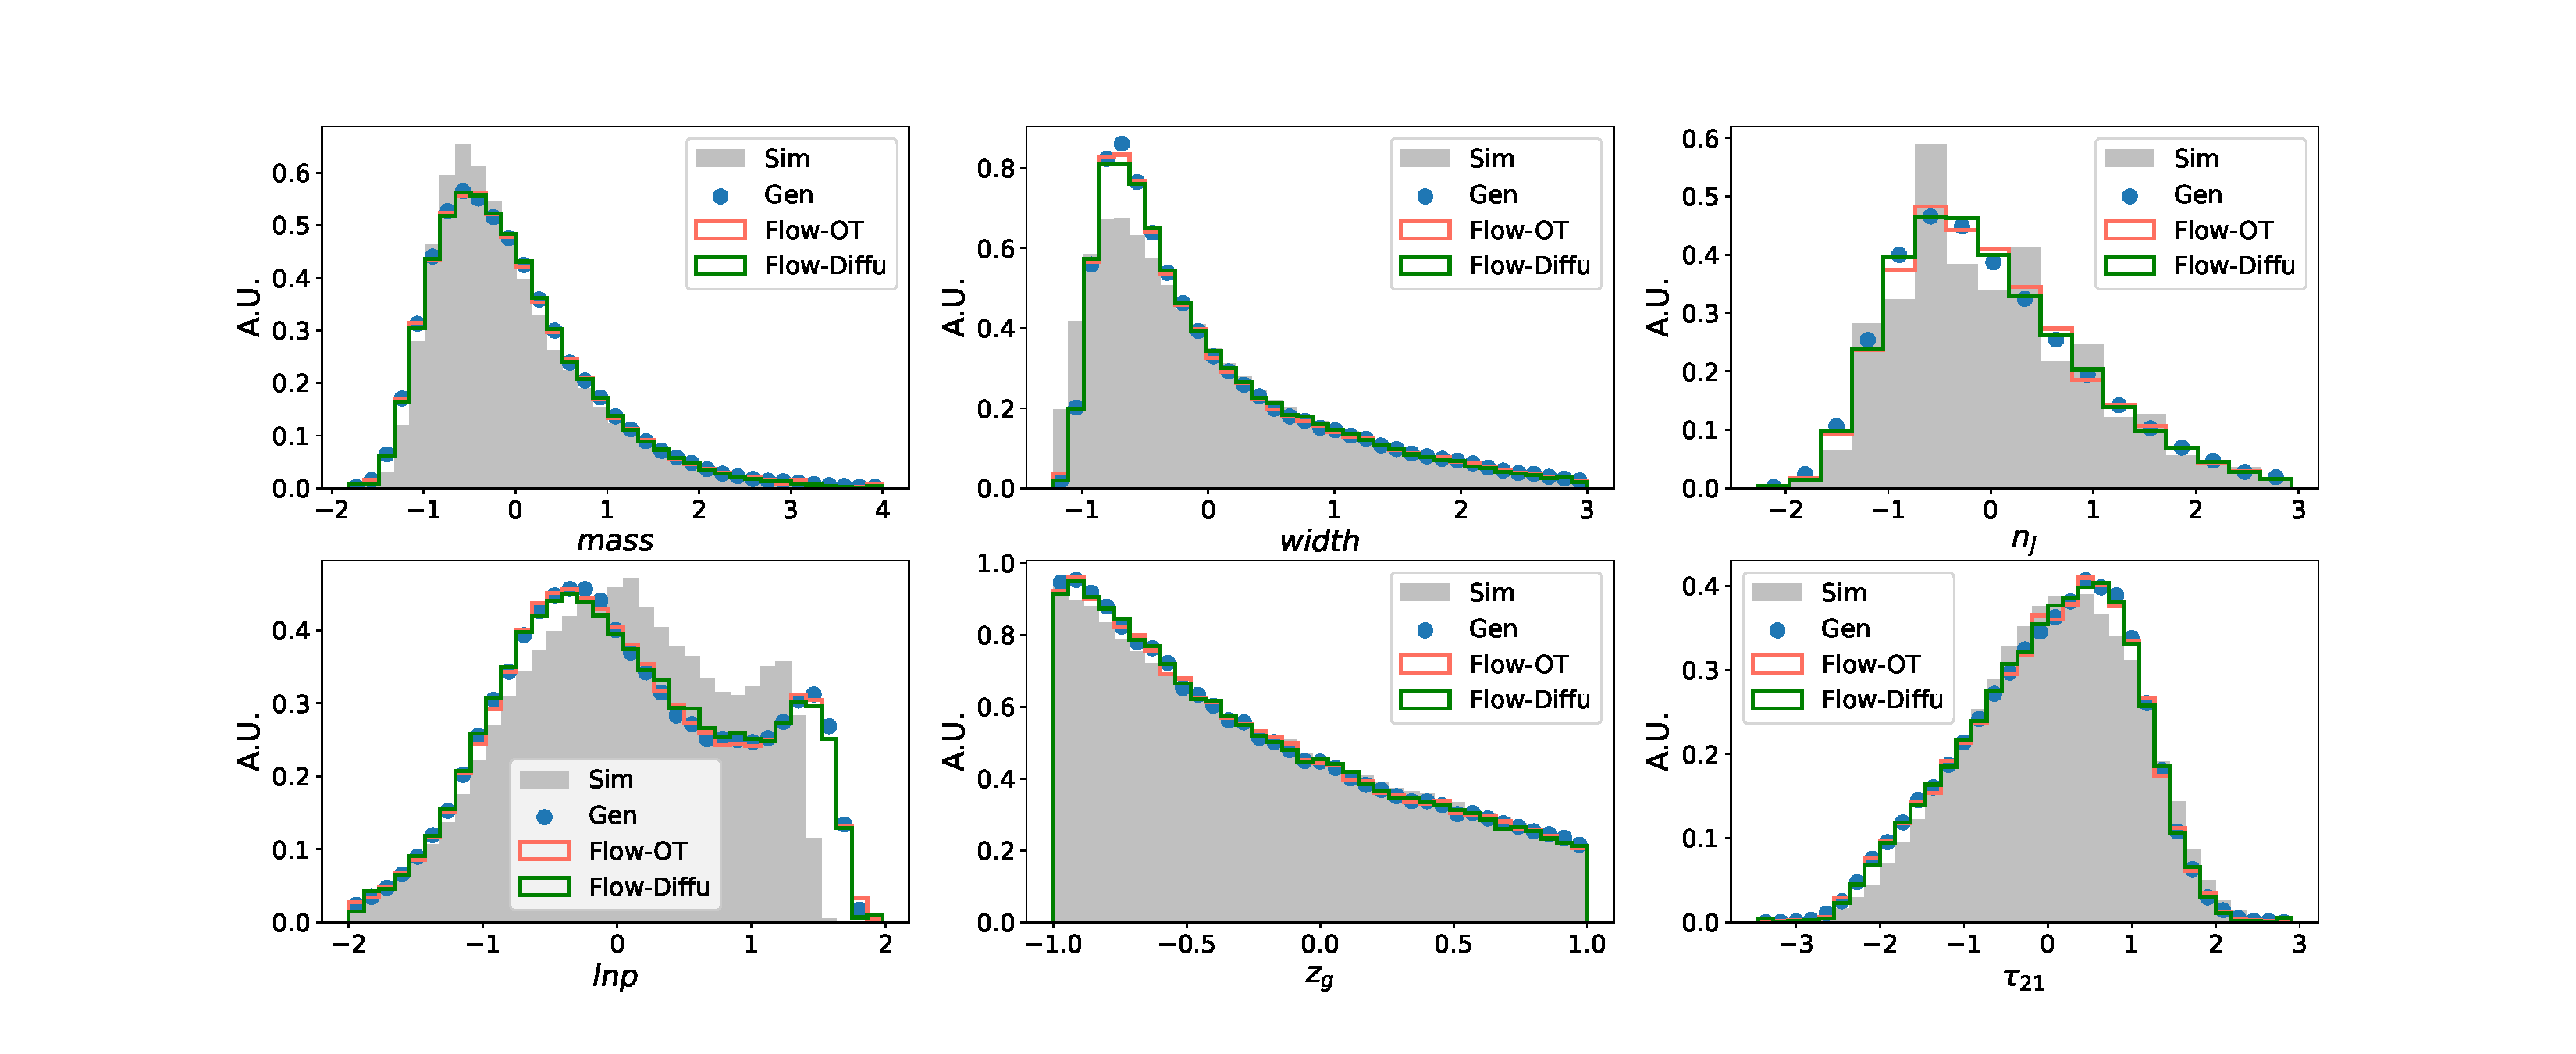
\includegraphics[width=\linewidth]{FLOWBDT/figures1/flowbdt_plot/fold_comp.pdf}
    \caption{Comparison plots of the histograms for 6 observables from leading jets for unfolding. Flow-Diffu: from Gaussian prior, Flow-OT: from conditioned prior, Gen: target unfolded observables, Sim: from reconstructed events.}
    \label{fig8}
\end{figure*}

\begin{figure*}[htbp]
    \centering
    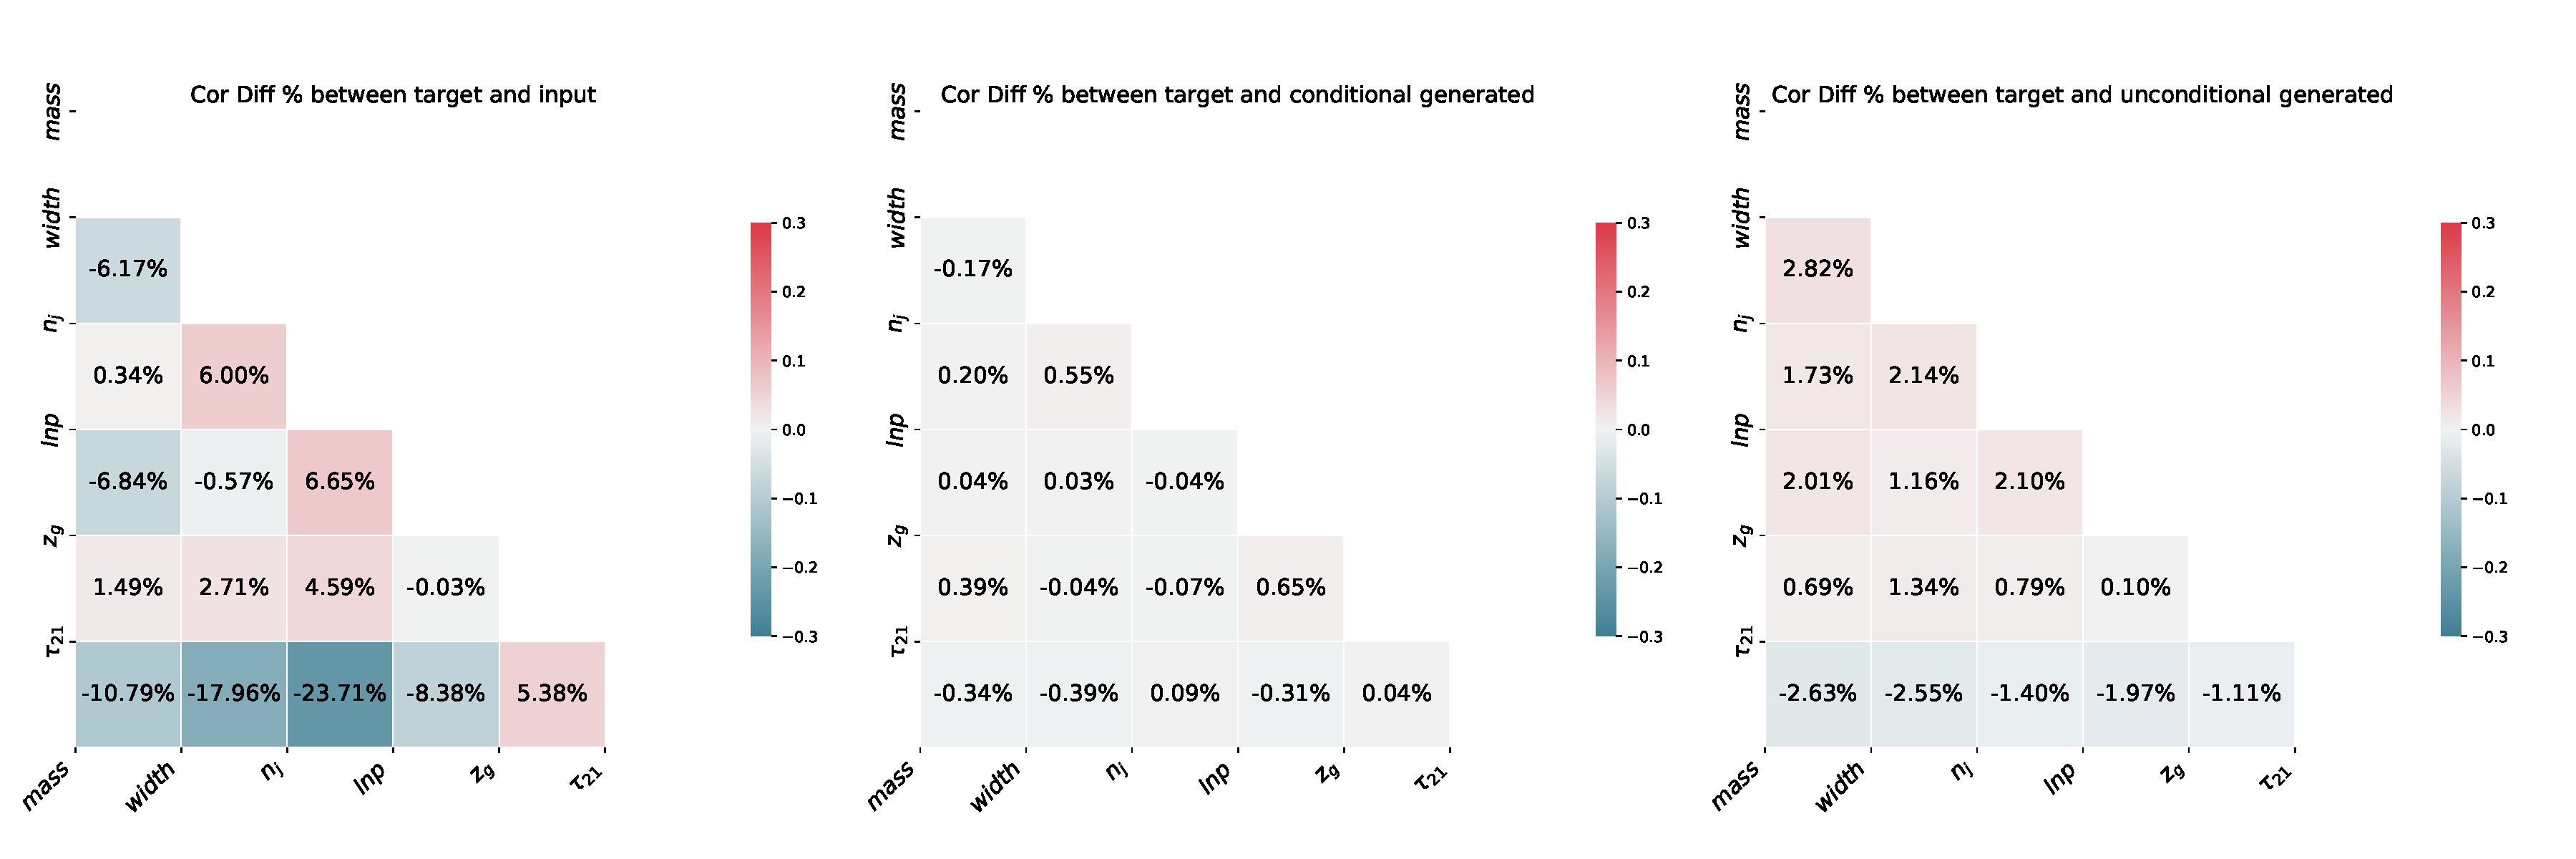
\includegraphics[width=\linewidth]{FLOWBDT/figures1/flowbdt_plot/fold_cor.pdf}
    \caption{Comparison plots of the correlation difference heatmaps for 6 observables from leading jets for unfolding. Left: Between target data and original simulation level input, middle: Between target data and generation from conditioned prior, right: Between target data and generation from Gaussian prior. }
    \label{fig9}
    
\end{figure*}


\begin{table*}[htbp]
    \centering
    \begin{ruledtabular}
        \begin{tabular}{cccc}
        \textbf{Observables} (Sep$\times$100 / W1$\times$10) & \textbf{Simulation} & \textbf{Conditional} & \textbf{Unconditional} \\ \hline
        \textbf{Jet mass} & $0.50 \pm 0.06$ / $0.37 \pm 0.03$ & $\mathbf{0.07 \pm 0.02}$ / $\mathbf{0.04 \pm 0.01}$ & $0.09 \pm 0.02$ / $0.08 \pm 0.02$ \\
        \textbf{Jet width} & $1.77 \pm 0.10$ / $0.41 \pm 0.03$ & $0.04 \pm 0.02$ / $\mathbf{0.03 \pm 0.01}$ & $\mathbf{0.03 \pm 0.01}$ / $0.10 \pm 0.02$ \\
        \textbf{N constituents} & $1.13 \pm 0.08$ / $0.41 \pm 0.03$ & $0.10 \pm 0.03$ / $0.28 \pm 0.04$ & $\mathbf{0.07 \pm 0.02}$ / $\mathbf{0.26 \pm 0.04}$ \\
        \textbf{$\ln_{\rho}$} & $3.68 \pm 0.15$ / $0.92 \pm 0.05$ & $\mathbf{0.05 \pm 0.02}$ / $\mathbf{0.05 \pm 0.01}$ & $0.10 \pm 0.03$ / $0.08 \pm 0.02$ \\
        \textbf{$z_g$} & $0.05 \pm 0.02$ / $0.17 \pm 0.02$ & $\mathbf{0.01 \pm 0.01}$ / $\mathbf{0.03 \pm 0.01}$ & $0.01 \pm 0.01$ / $0.03 \pm 0.01$ \\
        \textbf{$\tau_{21}$} & $0.56 \pm 0.06$ / $0.59 \pm 0.04$ & $\mathbf{0.10 \pm 0.02}$ / $\mathbf{0.05 \pm 0.01}$ & $0.14 \pm 0.03$ / $0.09 \pm 0.02$ \\
            \end{tabular}
    \end{ruledtabular}

    \caption{Comparison of evaluation metrics over binned (separation power) and unbinned (Wasserstein-1) distributions of 6 unfolding observables. Uncertainties estimated via bootstrap resampling ($n=100$). Bold indicates the best generative model result for each metric.}
    \label{table1}
\end{table*}

\subsection{Schr{\"o}dinger Bridge Refinement}\label{subsec4.4}

The model is also utilized to refine and simulate calorimeter showers. The conditional input is derived from parameterized shower approximations produced by fast simulations. In typical machine learning models, we often use discrete conditions such as energy and coordinates for training. However, some attributes, such as material type, are difficult to define numerically. Using an approximate shower as a condition offers a novel way to integrate these factors to guide the model with more explicit information inside the calorimeter.


Again, we flatten the calorimeter cells before training. Although this increases the training time compared to tasks with fewer dimensions, the computational cost is still generally smaller than most models we have encountered. Figure~\ref{fig10} shows the histogram of the deposited energy sum for the electron shower. The generated histogram displays a peak width very similar to the original, but with sharper tails at the lower energy end.


\begin{figure}[htbp]
    \centering
    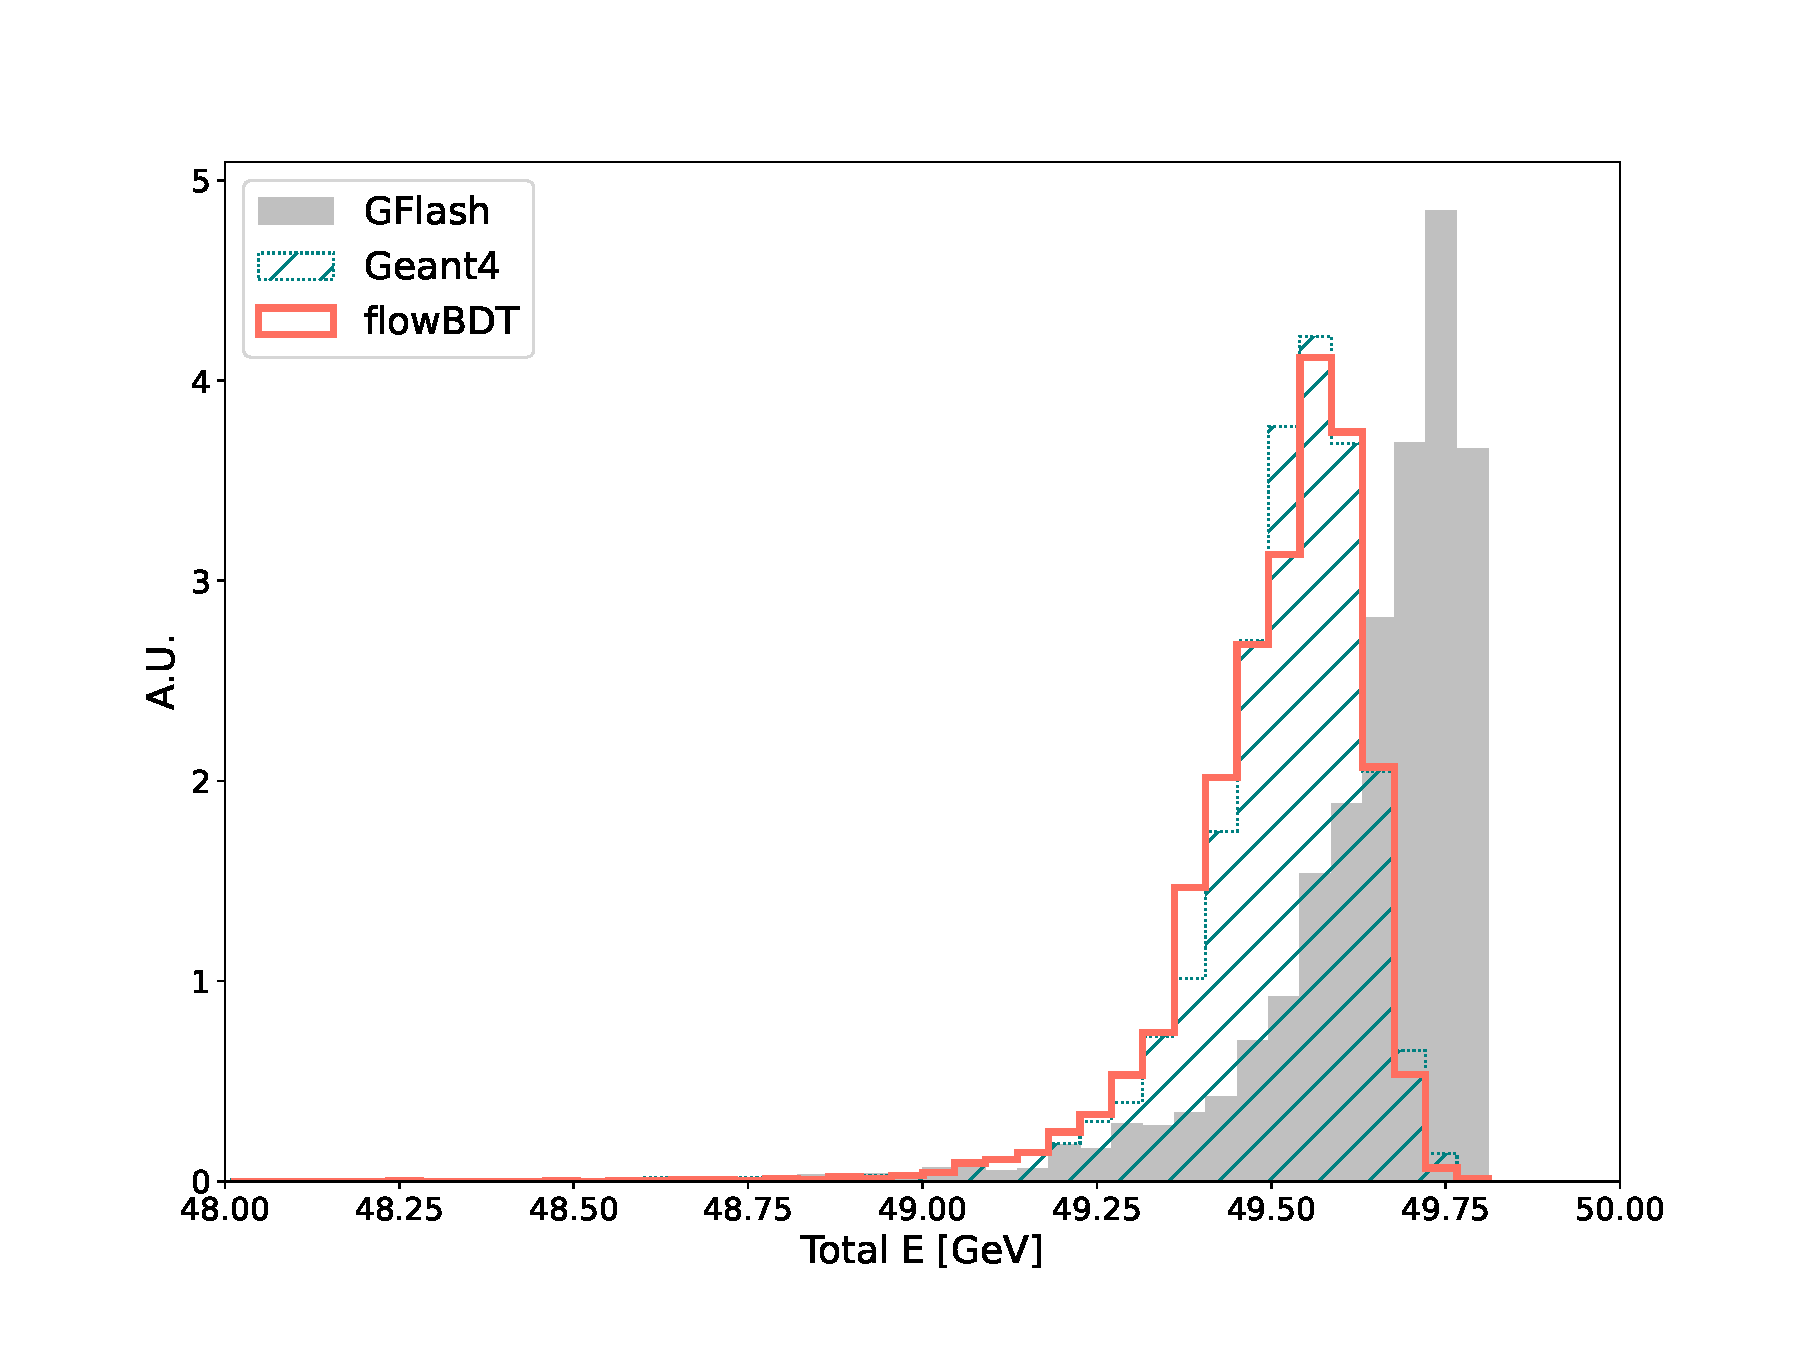
\includegraphics[width=0.4\textwidth]{FLOWBDT/figures1/flowbdt_plot/sb_sume.pdf}
    \caption{Total energy deposited for 50 GeV electron shower in the 10 * 10 calorimeter. GFlash: from classical fast simulation, flowBDT: generated sample, Geant4: from full simulation}
    \label{fig10}
\end{figure}


\section{Conclusion and outlooks}\label{sec5}

In this work, we have introduced BUFF, a framework applying conditional flow matching with Gradient Boosted Trees to various HEP tasks at different analysis levels. The flowBDT model features several enhancements over the original approach of~\cite{flowbdt}: the use of higher-order ODE solvers to reduce the number of sampling steps, a multi-output tree strategy yielding a 5--8$\times$ speedup in inference, and conditional generation from non-Gaussian priors. The lightweight GBT models achieve negligible inference time, significantly shortening generation for high-level tasks compared to traditional neural network-based flow matching. BUFF is well suited for rapid parallel training across multiple CPU cores.

We evaluated the generated high-level features for complex top jet topologies using both the triangular discriminator and Wasserstein-1 distance with bootstrap uncertainties, finding the marginal distributions to be reproduced to within $\sim\!2$--$5\times$ the finite-sample truth-baseline floor for most features. We extended the approach to much higher dimensions for the simulation of calorimeter voxels and jet constituents: per-feature marginals are reproduced to within a small multiple of the finite-sample truth floor, but jet--level kinematics derived from the 30$\times$3 representation remain three orders of magnitude above that floor (Table~\ref{tab2}), exposing the limitation of independent per-feature regression. Addressing this with a multi-output backbone or an explicit jet--level loss is a natural follow-up. We further demonstrated the advantages of conditional generation: for unfolding, the relative improvement in correlation agreement with the target is over 30 times higher when starting from a reconstructed-level prior. Conditional generation can also be applied to calorimeter shower refinement, using approximate showers that encode geometry and material information.

Looking ahead, we plan to extend BUFF to additional tasks such as anomaly detection and quark-gluon tagging. For low-level simulations, we will explore strategies to further enhance efficiency. The code for training, sampling, and evaluation, including the bootstrap, classifier, and consistency-check evaluation pipelines used for this revision, is publicly available at \url{https://github.com/DickyChant/BUFF}.

\section{Acknowledgements}

We would like to thank Jie Xiao for his insightful inputs on the study of conditional generation, and Dominik Duda for discussion on realistic application scenarios under the context of the ATLAS experiment.%and Dominik Duda for considering the potential to develop and utilize models in the ATLAS analysis.


\begin{appendix}
\section{Sampling time metric}\label{secA1}

Fig.~\ref{fig11} illustrates how the batch size of generated samples should be chosen for different dimensionalities. Since multiple GBT models are loaded during the sampling stage, each model incurs a small initialization overhead. This overhead is non-negligible when the per-event sampling time is already below the millisecond scale, causing small batch sizes to result in disproportionately large per-event sampling times. For example, the total generation time scales by only a factor of 2 when increasing from 100 to 1000 events, and by a factor of 4--5 when scaling from 1000 to 10,000 events. This demonstrates the model's efficient scaling behavior, which is crucial for processing large datasets. Notably, the multi-output tree strategy results in faster inference, particularly at higher dimensions. As shown in the right panel of Fig.~\ref{fig11}, an event with 368 features consumes only 2.5 times more CPU time than an event with 90 features.

\begin{figure*} [htbp]
    \centering
        \centering
            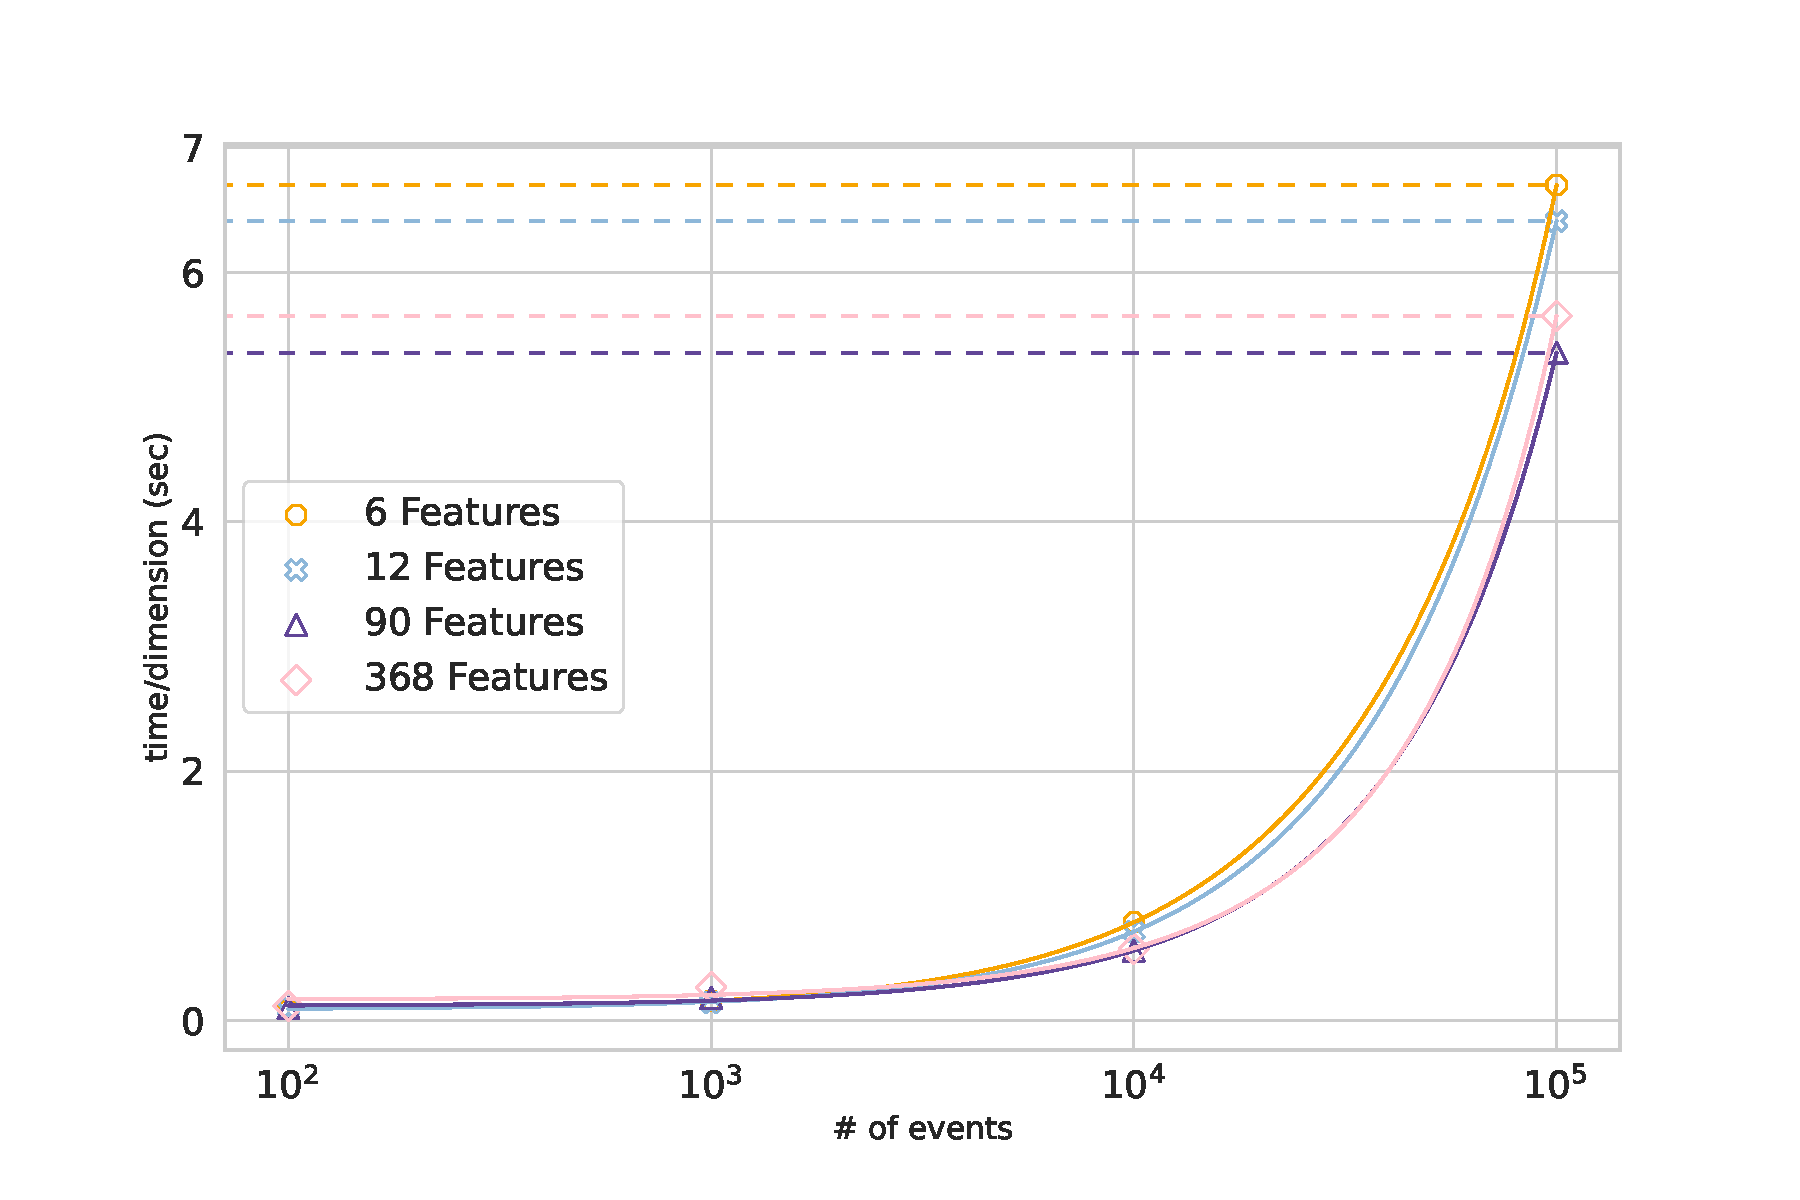
\includegraphics[width=0.4\textwidth]{FLOWBDT/figures1/flowbdt_plot/timedim.pdf}
            \quad\quad\quad
            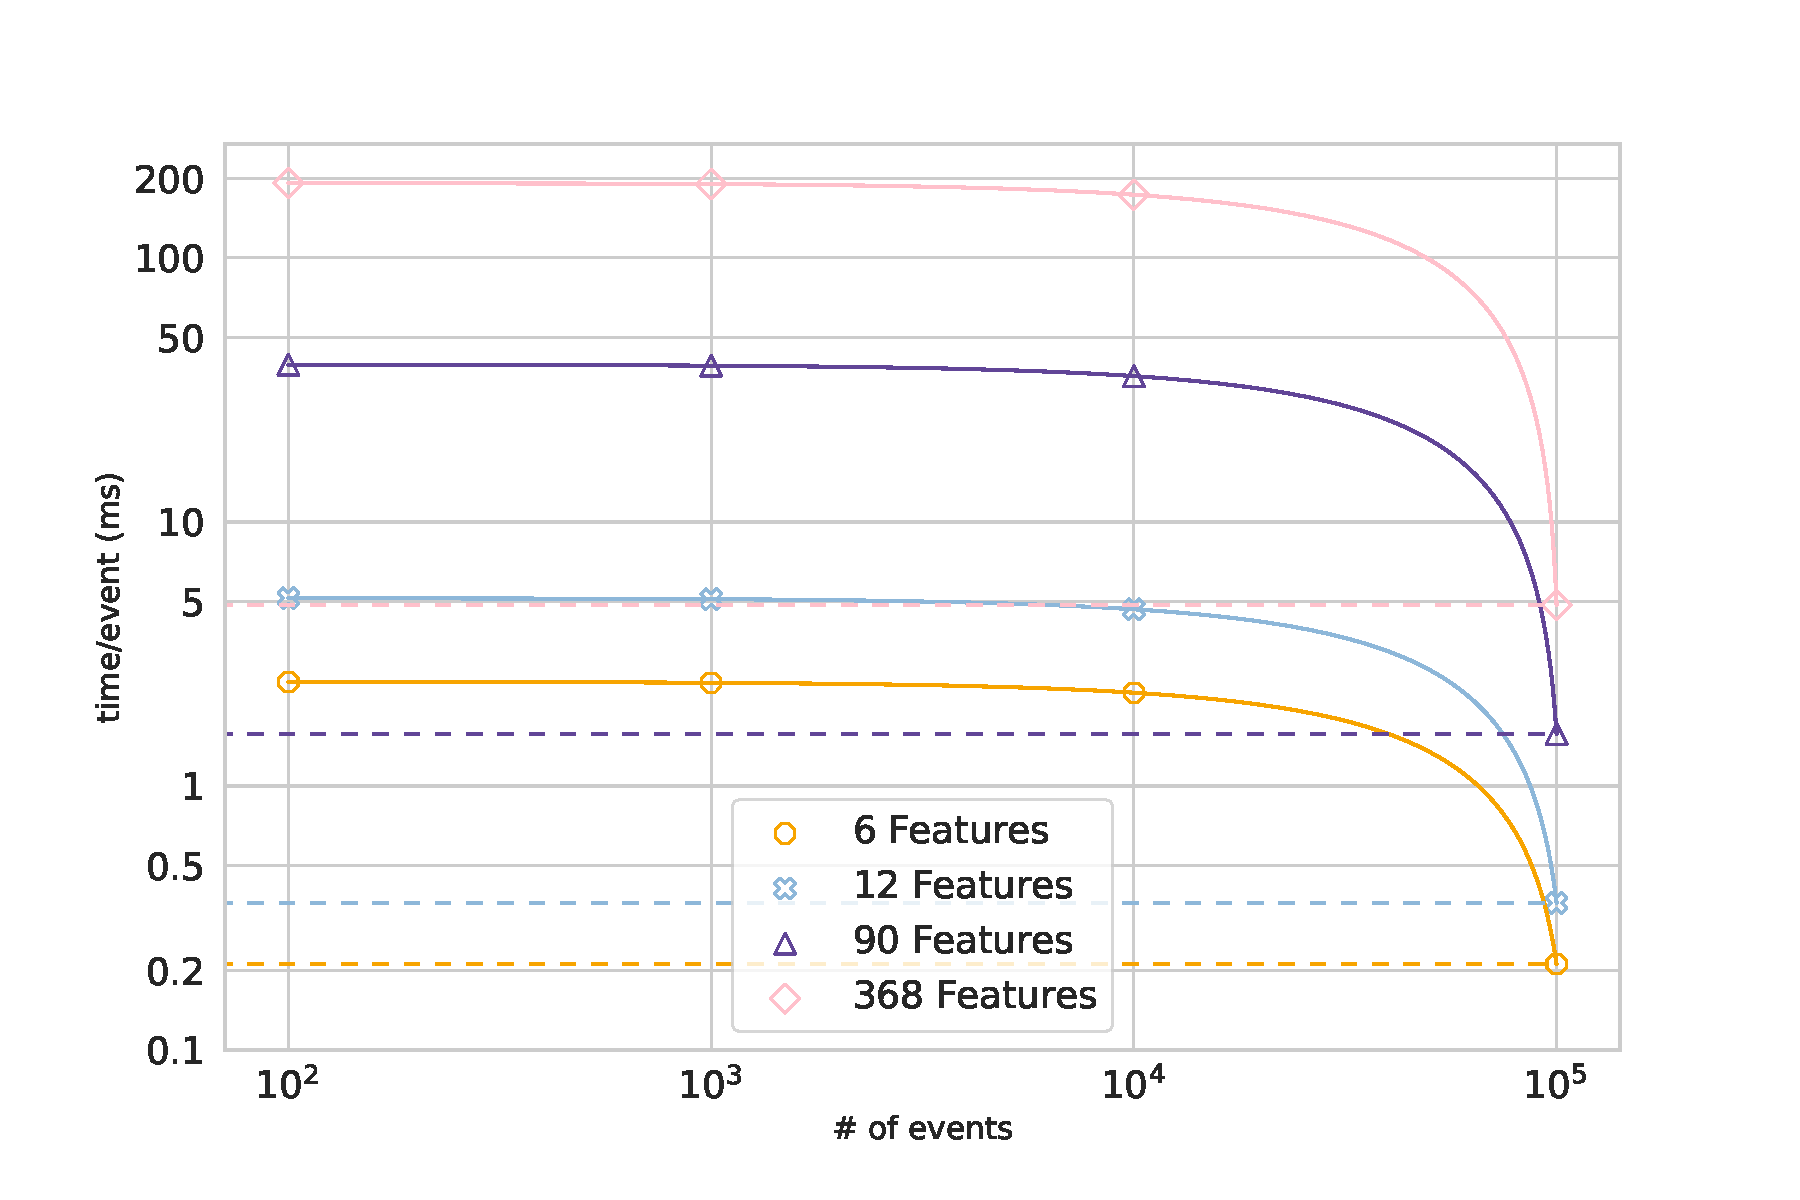
\includegraphics[width=0.4\textwidth]{FLOWBDT/figures1/flowbdt_plot/timeevent.pdf}
        \caption{Sampling time per feature (left) and per event (right) for number of events generated at once with different dimensionalities.}
        \label{fig11}
\end{figure*}

\end{appendix}

\newpage

\bibliography{prd.bib}

\end{document}
